\subsection{表示}

定义 1. 设 \(\mathfrak{g}\) 是 \(\mathbf{K}\) 上的李代数，\(\mathbf{M}\) 是一个 \(\mathbf{K}\) -模。从 \(\mathfrak{g}\) 到李代数 \(\mathfrak{gl}(\mathbf{M})\) 的同态称为 \(\mathfrak{g}\) 在模 \(\mathbf{M}\) 上的表示。单射表示称为忠实表示。如果 \(\mathbf{K}\) 是域，则 \(\mathbf{M}\) 在 \(\mathbf{K}\) 上的维数（有限或无限）称为该表示的维数。\(x \mapsto \operatorname{ad} x\) 在 \(\mathfrak{g}\) -模 \(\mathbf{K}\) 上的表示 \(\mathfrak{g}\) 称为 \(\mathfrak{g}\) 的伴随表示。

因此，g 在 M 上的表示是从 g 到 M 的自同态模的 K-线性映射 \(\rho\)，满足

\[
\rho ([ x, y ]). m = \rho (x) \rho (y). m - \rho (y) \rho (x). m
\]

对所有 \(x \in g, y \in g, m \in M.\)

*例. 设 G 是实李群，g 是其李代数，\(\rho\) 是 G 在有限维实向量空间 E 上的解析表示。那么，相应的从 g 到 gl(E) 的同态就是 g 在 E 上的表示。*

设 \(\mathbf{U}\) 是 \(\mathfrak{g}\) 的包络代数。第 §2 节第 1 号的命题 1 在 \(\mathfrak{g}\) 在 \(\mathbf{M}\) 上的表示与 \(\mathbf{U}\) 在 \(\mathbf{M}\) 上的表示的集合之间建立了一一对应。另一方面，我们知道（《代数》，第 VIII 章，§13，第 1 号），结合代数 \(\mathbf{U}\) 的表示这一概念与左 \(\mathbf{U}\)-模这一概念等价。

定义 2. 设 g 是 K 上的李代数，U 是其包络代数。U 上的有单位元左模称为左 g-模，或简称 g-模。

若 M 是 g-模且 \(x \in U\)，则以 \(x_{M}\) 表示由 x 在 M 上定义的自同态（参见《代数》，第 VIII 章，§ 1，第 2 号）。

U 上的有单位元右模称为右 g-模。这样的模可与左 \(U^{0}\)-模等同，即（§2，第 4 号）可与左 \(g^{0}\)-模等同。

设 \(\phi\) 是 U 的主反自同构。如果 M 是右 g-模，则在 M 上规定左 g-模结构，写作 \(a.m = m.\phi (a)\)，其中 \(m\in \mathbf{M}\)，\(a\in \mathrm{U}\)。

模论中的概念和结果可以翻译成表示的语言：

\begin{enumerate}
\def\labelenumi{(\arabic{enumi})}
\tightlist
\item
  \(\rho\) 在 \(\rho'\) 和 \(\mathfrak{g}\) 上的两个表示 \(\mathbf{M}\) 和 \(\mathbf{M}'\)，当 \(\mathfrak{g}\)-模 \(\mathbf{M}\) 和 \(\mathbf{M}'\) 同构时，称为相似的或同构的。为此，当且仅当存在一个从 K-模 \(u\) 到 K-模 \(\mathbf{M}\) 的同构 \(\mathbf{M}'\)，使得
\end{enumerate}

\[
\rho^ {\prime} (x) = u \circ \rho (x) \circ u ^ {- 1}
\]

对所有 \(x \in g\)。

\begin{enumerate}
\def\labelenumi{(\arabic{enumi})}
\setcounter{enumi}{1}
\item
  对所有 \(i \in I\)，设 \(\rho_{i}\) 是 g 在 \(M_{i}\) 上的表示。令 M 为各 g-模 \(M_{i}\) 的直和所成的 g-模。相应地有 g 在 M 上的表示 \(\rho\)，称为各 \(\rho_{i}\) 的直和，记作 \(\sum_{i\in I}\rho_{i}\)（当有 n 个表示 \(\rho_{1} + \cdots + \rho_{n}\) 时也记作 \(\rho_{1}, \ldots, \rho_{n}\)）。若 \(m = (m_{i})_{i \in I}\) 是 M 的元素且 \(x \in g\)，则 \(\rho(x).m = (\rho_{i}(x).m_{i})_{i \in I}\)。
\item
  \(\rho\) 在 \(\mathfrak{g}\) 上的表示 \(\mathbf{M}\)，当相应的 \(\mathfrak{g}\)-模是简单模时，称为简单的或不可约的。就是说，\(\mathbf{M}\) 中不存在在所有 \(\{0\}\)（\(\mathbf{M}\)）下稳定的子 K-模（除 \(\rho(x)\) 和 \(x \in \mathfrak{g}\) 外）。一类简单 \(\mathfrak{g}\)-模（《代数》，第 VIII 章，§ 3，第 2 号）定义了 \(\mathfrak{g}\) 的一类简单表示。
\item
  \(\rho\) 是 \(\mathfrak{g}\) 在 \(\mathbf{M}\) 上的表示；当相应的 \(\mathfrak{g}\)-模是半单模时，称其为半单的或完全可约的。这等价于说，\(\rho\) 与简单表示的直和相似，或者每个子 K-模
\end{enumerate}

M 在 \(\rho(x)\)（\(x \in \mathfrak{g}\)）下稳定，都有一个在 \(\rho(x)\)（\(x \in \mathfrak{g}\)）下稳定的补模（参见《代数》，第 VIII 章，§ 3，第 3 号）。

\begin{enumerate}
\def\labelenumi{(\arabic{enumi})}
\setcounter{enumi}{4}
\item
  设 \(\delta\) 是 \(\mathfrak{g}\) 的一类简单表示，对应于一类简单 \(\mathfrak{g}\)-模 C。另一方面，设 \(\rho\) 是 \(\mathfrak{g}\) 在 M 上的表示。\(\mathrm{M}_{\mathbb{C}}\)-模 M 的 C 型等型分量 \(\mathfrak{g}\)（《代数》，第 VIII 章，§ 3，第 4 号）也称为 M 的 \(\delta\) 型等型分量。该分量是 M 中所有在 \(\rho(x)\) 下稳定且 \(\rho(x)\) 在其上诱导出 \(\delta\) 类表示的子 K-模之和；它是其中某些子模的直和；若 \(\mathrm{M}_{\mathbb{C}}\) 的长度为 \(n\)，则称 \(\rho\) 含有 \(\delta\) 个 \(n\)。不同 \(\mathrm{M}_{\mathbb{C}}\) 的和是直和；当且仅当 \(\rho\) 半单时，它等于 M。
\item
  设 \(\rho, \rho'\) 是 \(\mathfrak{g}\) 的两个表示。如果 \(\rho'\) 的模是 \(\rho\) 的模的子模（分别为商模），则称 \(\rho'\) 是 \(\rho\) 的子表示（分别为商表示）。
\end{enumerate}

设 M 是 K-模。g 在 M 上的零表示在 M 上定义了 g-模结构。赋予此结构的 M 称为平凡 g-模。

设 M 是 g-模。M 的子 g-模的商 g-模也都是 M 的商模的子 g-模：它们由 M 的两个子 g-模 U、U'（满足 U ⊃ U'）以及 g-模 U/U' 得到。若上述类型的所有简单模都同构于给定的简单 g-模 N，则称 M 为 N 型纯 g-模。若 ρ 和 σ 是分别对应于 M 和 N 的 g 表示，也说 ρ 是 σ 型纯表示。

设 \(M'\) 是 M 的子 g-模。M 是 N 型纯模的充要条件是 \(M'\) 和 \(M/M'\) 都是 N 型纯模。必要性显然。设此条件成立，令 U、\(U'\) 是 M 的子 g-模，满足 \(U' \subset U\) 且 \(U/U'\) 简单；令 \(\phi\) 是从 M 到 \(M/M'\) 的典范同态；若 \(\phi(U) \neq \phi(U')\)，则 \(U/U'\) 同构于 \(\phi(U)/\phi(U')\)，因而同构于 N；若 \(\phi(U) = \phi(U')\)，则 \(U \subset U' + M'\)，所以 \(U/U'\) 同构于 \((U' + M')/U'\) 的一个简单子模，而后一个模又同构于 \(M'/(U' \cap M')\)；故 \(U/U'\) 再次同构于 N，从而 M 是 N 型纯模。

以下设 M 是 g-模，并假设 M 的 N 型纯子 g-模的集合有最大元 \(M'\)。那么，M 的每个 N 型纯子模 \(M''\) 都包含于 \(M'\) 中。因为 \(M''/(M' \cap M'')\) 和 \(M'\) 都是 N 型纯模，所以上述结果表明 \(M' + M''\) 是 N 型纯模，从而 \(M' + M'' \subset M'\)。

假设 g-模 M 有一个 Jordan-Hölder 序列 \((\mathrm{M}_{1})_{0\leqslant i\leqslant n}\)。M 是 N 型纯模的充要条件是 \(M_{0}/M_{1}\)、\(M_{1}/M_{2}\)、\(\ldots\)、\(M_{n-1}/M_{n}\) 都同构于 N；必要性显然，而充分性由上述结果对 n 作归纳立即得到。

命题 1. 设 g 是 K 上的李代数，a 是 g 的理想。设 M 是 g-模，N 是简单 a-模。把 M 看作 a-模，并假设 M 的 N 型纯子 a-模的集合有最大元 M'。则 M' 是 M 的子 g-模。

设 \(y \in \mathfrak{g}\)。令 \(\phi\) 为从 M 到 \(M / M'\) 的典范映射，令 \(f\) 为从 \(m \mapsto \phi(y_M. m)\) 到 \(M'\) 的映射 \(M / M'\)。只需证明 \(f(M') = \{0\}\)。设 \(x \in \mathfrak{a}\)。则对 \(m \in M\)，

\[
x _ {\mathrm{M} / \mathrm{M} ^ {\prime}}. f (m) = \phi (x _ {\mathrm{M}} y _ {\mathrm{M}}. m) = \phi (y _ {\mathrm{M}} x _ {\mathrm{M}}. m) + \phi ([ x, y ] _ {\mathrm{M}}. m).
\]

现在 \([x,y] \in \mathfrak{a}\)，从而 \(\phi([x,y]_{\mathbb{M}}.m) = 0\)；另一方面，

\[
\phi (y _ {\mathrm{M}} x _ {\mathrm{M}}. m) = f (x _ {\mathrm{M}}. m).
\]

因此 \(x_{\mathbf{M} / \mathbf{M}'} . f(m) = f(x_{\mathbf{M}}.m)\)。于是 \(f(\mathbf{M}')\) 是 \(\mathbf{M} / \mathbf{M}'\) 的子 a-模，并同构于 \(\mathbf{M}'\) 的一个商模，因而是 \(\mathbf{N}\) 型纯模；所以 \(f(\mathbf{M}') = \{0\}\)。

推论。设 g 是 K 上的李代数，a 是 g 的理想。设 M 是简单 g-模，并且作为 K-模具有有限长度。则存在简单 a-模 N，使得 M 是 N 型纯 a-模。

由于 \(a\)-模 \(\mathbf{M}\) 具有有限长度，\(\mathbf{N}\) 的子 \(a\)-模集合中存在极小元 \(\mathbf{M}\)：它是 \(a\) 的简单子 \(\mathbf{M}\)-模。因此，\(a\) 中最大的 \(\mathbf{M}\) 型纯子 \(\mathbf{N}\)-模不等于 \(\neq \{0\}\)，并且是 \(g\) 的子 \(\mathbf{M}\)-模（命题 1），所以它必等于 \(\mathbf{M}\)。

\subsection{表示的张量积}

我们在第 1 号中定义了 g 的一族表示的直和。现在定义表示的其他运算。

设 \(\mathfrak{g}_1, \mathfrak{g}_2\) 是 \(\mathbf{K}\) 上的两个李代数，\(\mathbf{M}_i\) 是一个 \(\mathfrak{g}_i\)-模（\(i = 1, 2\)）。令 \(\mathbf{U}_i\) 为 \(\mathfrak{g}_i\) 的包络代数，\(\sigma_i\) 为从 \(\mathfrak{g}_i\) 到 \(\mathbf{U}_i\) 的典范映射。于是 \(\mathbf{M}_i\) 是左 \(\mathbf{U}_i\)-模，因而 \(\mathbf{M}_1 \otimes_{\mathbf{K}} \mathbf{M}_2\) 具有典范的左 \((\mathbf{U}_1 \otimes_{\mathbf{K}} \mathbf{U}_2)\)-模结构。现在 \(\mathbf{U}_1 \otimes_{\mathbf{K}} \mathbf{U}_2\) 是 \(\mathfrak{g}_1 \times \mathfrak{g}_2\) 的包络代数，而映射 \((x_1, x_2) \mapsto \sigma_1(x_1) \otimes 1 + 1 \otimes \sigma_2(x_2)\) 是从 \(\mathfrak{g}_1 \times \mathfrak{g}_2\) 到此包络代数的典范映射（§ 2，第 2 号）。因此，在 \((\mathfrak{g}_1 \times \mathfrak{g}_2)\) 上存在 \(\mathbf{M} = \mathbf{M}_1 \otimes_{\mathbf{K}} \mathbf{M}_2\)-模结构，使得：

\[
\begin{array}{r l} (x _ {1}, x _ {2}) _ {\mathrm{M}}. (m _ {1} \otimes m _ {2}) & = (\sigma_ {1} (x _ {1}) \otimes 1 + 1 \otimes \sigma_ {2} (x _ {2})) . (m _ {1} \otimes m _ {2}) \\ & = ((x _ {1}) _ {\mathrm{M} _ {1}}. m _ {1}) \otimes m _ {2} + m _ {1} \otimes ((x _ {2}) _ {\mathrm{M} _ {2}}. m _ {2}). \end{array}\tag{1}
\]

此结构定义了 \(\mathfrak{g}_1\times \mathfrak{g}_2\) 在 \(\mathbf{M}\) 上的表示。

若现在 \(\mathfrak{g}_1 = \mathfrak{g}_2 = \mathfrak{g}\)，则从 \(x \mapsto (x, x)\) 到 \(\mathfrak{g}\) 的同态 \(\mathfrak{g} \times \mathfrak{g}\) 与上述表示复合，定义了 \(\mathfrak{g}\) 在 \(\mathbf{M}\) 上的表示，因而在 \(\mathfrak{g}\) 上定义了 \(\mathbf{M}\)-模结构，使得：

\[
x _ {\mathrm{M}}. (m _ {1} \otimes m _ {2}) = (x _ {\mathrm{M} _ {1}}. m _ {1}) \otimes m _ {2} + m _ {1} \otimes (x _ {\mathrm{M} _ {2}}. m _ {2}).\tag{2}
\]

同理可见：

命题 2. 设 g 是 K 上的李代数，\(M_{i}\) 是 g-模（\(1 \leqslant i \leqslant n\)）。在张量积 \(M_{1} \otimes_{K} M_{2} \otimes \cdots \otimes M_{n}\) 上存在唯一的 g-模结构，使得

\[
x _ {\mathrm{M}}. (m _ {1} \otimes \dots \otimes m _ {n}) = \sum_ {i = 1} ^ {n} m _ {1} \otimes \dots \otimes (x _ {\mathrm{M} _ {i}}. m _ {i}) \otimes \dots \otimes m _ {n}\tag{3}
\]

对所有 \(x \in \mathfrak{g}\)、\(m_1 \in \mathbf{M}_1, \ldots, m_n \in \mathbf{M}_n\)。

相应的表示称为给定的 g 在各 \(M_{i}\) 上的表示的张量积。

特别地，若 \(\mathbf{M}\) 是 \(\mathfrak{g}\)-模，命题 2 定义了 \(\mathfrak{g}\)-模结构
在每个 \(\mathbf{M}_p = \bigotimes \mathbf{M}\) 上定义了结构，因而也在 \(\mathbf{T}\) 的张量代数 \(\mathbf{M}\) 上定义了结构。

公式 (3) 表明，对所有 \(x \in \mathfrak{g}\)，\(x_{\mathrm{T}}\) 是代数 \(\mathrm{T}\) 上延拓 \(x_{\mathrm{M}}\) 的唯一导子。我们知道（§ 2，第 8 号），\(x_{\mathrm{T}}\) 在取商后在 \(\mathrm{S}\) 的对称代数 \(\mathrm{M}\) 上定义了一个导子。因此，可以把 \(\mathrm{S}\) 看作 \(\mathfrak{g}\) 的商 \(\mathrm{T}\)-模，而 \(x_{\mathrm{S}}\) 是 \(\mathrm{S}\) 的导子。

更具体地，把 g 借助其伴随表示看作 g-模。设 U 是 g 的包络代数。根据 §2 的命题 7，\(x_{\mathrm{M}}\) 在取商后定义了 U 上的导子，而这正是由 \(\sigma(x)\) 定义的内导子（\(\sigma\) 表示从 g 到 U 的典范映射）。于是可以把 U 看作 T 的商 g-模。如果 K 是特征为 0 的域，则从 S 到 U 的典范同构是 g-模同构（§2，第 8 号）。

\subsection{同态模上的表示}

再次设 \(\mathfrak{g}_1\) 和 \(\mathfrak{g}_2\) 是 K 上的两个李代数，\(\mathbf{M}_i\) 是一个 \(\mathfrak{g}_i\)-模（\(i = 1, 2\)）。令 \(\mathrm{U}_i\) 为 \(\mathfrak{g}_i\) 的包络代数，\(\sigma_i\) 为从 \(\mathfrak{g}_i\) 到 \(\mathrm{U}_i\) 的典范映射。于是 \(\mathbf{M}_i\) 是左 \(\mathrm{U}_i\)-模，因而 \(\mathcal{L}_{\mathrm{K}}(\mathrm{M}_1, \mathrm{M}_2)\) 具有典范的左 \((\mathrm{U}_1^0 \otimes \mathrm{U}_2)\)-模结构。现在 \(\mathrm{U}_1^0 \otimes_{\mathrm{K}} \mathrm{U}_2\) 是 \(\mathfrak{g}_1^0 \times \mathfrak{g}_2\) 的包络代数，映射

\[
(x _ {1}, x _ {2}) \mapsto \sigma_ {1} (x _ {1}) \otimes 1 + 1 \otimes \sigma_ {2} (x _ {2})
\]

是从 \(\mathfrak{g}_1^0\times \mathfrak{g}_2\) 到此包络代数的典范映射。因此，在 \((\mathfrak{g}_1^0\times \mathfrak{g}_2)\) 上存在 \(\mathbf{M} = \mathcal{L}_{\mathbb{K}}(\mathbf{M}_1,\mathbf{M}_2)\)-模结构，使得

\[
\begin{array}{r l} ((x _ {1}, x _ {2}) _ {\mathrm{M}}. u) \cdot m _ {1} & = ((\sigma_ {1} (x _ {1}) \otimes 1 + 1 \otimes \sigma_ {2} (x _ {2})) \cdot u) \cdot m _ {1} \\ & = u ((x _ {1}) _ {\mathrm{M} _ {1}}. m _ {1}) + (x _ {2}) _ {\mathrm{M} _ {2}}. u (m _ {1}) \end{array}\tag{4}
\]

对所有 \(u \in \mathcal{L}_{\mathbb{K}}(\mathrm{M}_1, \mathrm{M}_2)\)、\(m_1 \in \mathrm{M}_1\) 均成立。此结构定义了 \(\mathfrak{g}_1^0 \times \mathfrak{g}_2\) 在 \(\mathbf{M}\) 上的表示。

若现在 \(\mathfrak{g}_1 = \mathfrak{g}_2 = \mathfrak{g}\)，则从 \(x \mapsto (-x, x)\) 到 \(\mathfrak{g}\) 的同态 \(\mathfrak{g}^0 \times \mathfrak{g}\) 与上述表示复合，定义了 g 在 M 上的表示，因而在 M 上定义了 g-模结构，使得

\[
(x _ {\mathrm{M}}. u). m _ {1} = x _ {\mathrm{M} _ {2}}. u (m _ {1}) - u (x _ {\mathrm{M} _ {1}}. m _ {1})\tag{5}
\]

或

\[
x _ {\mathrm{M}}. u = x _ {\mathrm{M} _ {2}} u - u x _ {\mathrm{M} _ {1}}.\tag{6}
\]

结合这些结果与命题 2，得到：

命题 3. 设 \(\mathfrak{g}\) 是 \(\mathbf{K}\) 上的李代数，\(\mathbf{M}_i\) 是 \(\mathfrak{g}\)-模（\(1 \leqslant i \leqslant n + 1\)）。

令 \(\mathbf{N}\) 为 K-模 \(\mathcal{L}_{\mathbf{K}}(\mathbf{M}_1, \ldots, \mathbf{M}_n; \mathbf{M}_{n+1})\)，即从 \(\prod_{i=1}^{n} \mathbf{M}_i\) 到 \(\mathbf{M}_{n+1}\) 的多重线性映射的 K-模。在 \(\mathbf{N}\) 上存在唯一的 g-模结构，使得

\[
\begin{array}{r l} (x _ {N}. u) (m _ {1}, \ldots , m _ {n}) & = - \sum_ {i = 1} ^ {n} u (m _ {1}, \ldots , x _ {M _ {i}}. m _ {i}, \ldots , m _ {n}) \\ & \quad + x _ {M _ {n + 1}}. u (m _ {1}, \ldots , m _ {n}) \end{array}\tag{7}
\]

对所有 \(x \in \mathfrak{g}\)、\(u \in \mathbf{N}\) 及 \(m_i \in \mathbf{M}_i\)（\(1 \leqslant i \leqslant n\)）成立。

特别地，设 g 是 K 上的李代数，M 是 g-模，并把 K 看作平凡 g-模。命题 3 在 \(\mathcal{L}_{\mathrm{K}}(\mathrm{M},\mathrm{K}) = \mathrm{M}^{*}\) 上定义了 g-模结构。相应的表示称为表示 \(x\mapsto x_{\mathrm{M}}\) 的对偶表示。我们有：

\[
(x _ {\mathrm{M} ^ {*}}. f) (m) = - f (x _ {\mathrm{M}}. m)\tag{8}
\]

对所有 \(x \in \mathfrak{g}, f \in \mathbf{M}^*\)、\(m \in \mathbf{M}\) 成立。换言之：

\[
x _ {\mathrm{M} ^ {*}} = - ^ {t} x _ {\mathrm{M}}.\tag{9}
\]

当 K 是域且 M 是有限维时，g-模 M 是简单的（分别为半单的），当且仅当 g-模 M* 是简单的（分别为半单的）。

命题 4. 设 \(\mathbf{M}_1, \mathbf{M}_2\) 是两个 g-模。典范的 K-线性映射（《代数》，第 II 章，§ 4，第 2 号命题 2 以及第 1 号命题 1）：

\[
\mathrm{M} _ {1} ^ {*} \otimes_ {\mathrm{K}} \mathrm{M} _ {2} \xrightarrow {\Phi} \mathscr {L} _ {\mathrm{K}} (\mathrm{M} _ {1}, \mathrm{M} _ {2}), \quad \mathscr {L} _ {\mathrm{K}} (\mathrm{M} _ {1}, \mathrm{M} _ {2} ^ {*}) \xrightarrow {\Psi} (\mathrm{M} _ {1} \otimes_ {\mathrm{K}} \mathrm{M} _ {2}) ^ {*}
\]

（其中第二个是双射）都是 \(\mathfrak{g}\)-模同态。

  记作

\[
\mathrm{N} = \mathrm{M} _ {1} ^ {*} \otimes \mathrm{M} _ {2}, \quad \mathrm{P} = \mathscr {L} (\mathrm{M} _ {1}, \mathrm{M} _ {2}), \quad \mathrm{Q} = \mathscr {L} (\mathrm{M} _ {1}, \mathrm{M} _ {2} ^ {*}), \quad \mathrm{R} = (\mathrm{M} _ {1} \otimes \mathrm{M} _ {2}) ^ {*}.
\]

于是，对 \(x \in \mathfrak{g}, f \in \mathbf{M}_1^*\)、\(m_1 \in \mathbf{M}_1\)、\(m_2 \in \mathbf{M}_2\)，

\[
\begin{array}{r l} & {((\phi x _ {\mathrm{N}}) (f \otimes m _ {2})). m _ {1} = (\phi (x _ {\mathrm{M} _ {1} ^ {*}} f \otimes m _ {2} + f \otimes x _ {\mathrm{M} _ {2}} m _ {2})). m _ {1}} \\ & {\qquad = \langle x _ {\mathrm{M} _ {1} ^ {*}} f, m _ {1} \rangle m _ {2} + \langle f, m _ {1} \rangle x _ {\mathrm{M} _ {2}} m _ {2}} \\ & {((x _ {\mathrm{P}} \phi) (f \otimes m _ {2})). m _ {1} = x _ {\mathrm{M} _ {2}} (\phi (f \otimes m _ {2}). m _ {1}) - \phi (f \otimes m _ {2}) (x _ {\mathrm{M} _ {1}} m _ {1})} \\ & {\qquad = \langle f, m _ {1} \rangle x _ {\mathrm{M} _ {2}} m _ {2} - \langle f, x _ {\mathrm{M} _ {1}} m _ {1} \rangle m _ {2}} \end{array}
\]

从而 \(\phi x_{\mathbf{N}} = x_{\mathbb{P}}\phi\)。另一方面，对 \(x \in \mathfrak{g}\)、\(u \in \mathcal{L}(\mathrm{M}_1, \mathrm{M}_2^*)\)、\(m_1 \in \mathrm{M}_1\)、\(m_2 \in \mathrm{M}_2\)：

\[
\begin{array}{r l} (\psi x _ {\mathbf {Q}} u) (m _ {1} \otimes m _ {2}) & = \langle (x _ {\mathbf {Q}} u). m _ {1}, m _ {2} \rangle = \langle x _ {\mathrm{M} _ {2} ^ {*}} u m _ {1} - u x _ {\mathrm{M} _ {1}} m _ {1}, m _ {2} \rangle \\ (x _ {\mathrm{R}} \psi u) (m _ {1} \otimes m _ {2}) & = - \langle \psi u, x _ {\mathrm{M} _ {1}} m _ {1} \otimes m _ {2} + m _ {1} \otimes x _ {\mathrm{M} _ {2}} m _ {2} \rangle \\ & = - \langle u x _ {\mathrm{M} _ {1}} m _ {1}, m _ {2} \rangle - \langle u m _ {1}, x _ {\mathrm{M} _ {2}} m _ {2} \rangle \end{array}
\]

从而 \(\psi x_{Q} = x_{R}\psi\)，命题得证。

在同构 \(\mathcal{L}(\mathrm{M}_1,\mathrm{M}_2^*)\) 下，g-模 \((\mathrm{M}_1\otimes \mathrm{M}_2)^*\) 与 \(\psi\) 等同。若 \(\mathbf{M}_1\) 和 \(\mathbf{M}_2\) 有限基，则 \(\phi\) 是同构（《代数》，第 II 章，§ 4，第 2 号命题 2），这使我们可以把 g-模 \(\mathbf{M}_1^*\otimes \mathbf{M}_2\) 与 \(\mathcal{L}(\mathrm{M}_1,\mathrm{M}_2)\) 等同；在这种情况下，我们还可以把 g-模 \(\mathbf{M}_1^*\otimes \mathbf{M}_2^*\)、\(\mathcal{L}(\mathrm{M}_1,\mathbf{M}_2^*)\) 与 \((\mathrm{M}_1\otimes \mathrm{M}_2)^*\) 等同。

\subsection{例}

例 1. 设 \(\mathfrak{g}\) 是 \(\mathbf{K}\) 上的李代数，\(\mathbf{M}\) 是 \(\mathfrak{g}\)-模。\(\mathfrak{g}\) 上的 \(\mathbf{M}\)-模结构与 \(\mathfrak{g}\) 上的平凡 \(\mathbf{K}\)-模结构，在由 \(\mathfrak{g}\) 上的双线性形式组成的 \(\mathbf{K}\)-模 \(N = \mathcal{L}(M, M; K)\) 上定义了 \(\mathbf{M}\)-模结构。于是

\[
(x _ {N}. \beta) (m, m ^ {\prime}) = - \beta (x _ {M}. m, m ^ {\prime}) + \beta (m, x _ {M}. m ^ {\prime})\tag{10}
\]

对所有 \(x \in \mathfrak{g}\)、\(m, m'\) 属于 \(\mathbf{M}\)、\(\beta \in \mathbf{N}\) 成立。若 \(\beta\) 是 \(\mathbf{N}\) 的给定元素，则满足 \(x \in \mathfrak{g}\) 的 \(x_{\mathbf{N}}. \beta = 0\) 的集合是 \(\mathfrak{g}\) 的子代数。

设 \(\mathbf{M}\) 是 K-模，\(\beta\) 是 \(\mathbf{M}\) 上的双线性形式。由上面所述，满足 \(x \in \mathfrak{gl}(\mathbf{M})\) 的

\[
\beta (x. m, m ^ {\prime}) + \beta (m, x. m ^ {\prime}) = 0
\]

对所有 \(m \in \mathbf{M}\) 和 \(m' \in \mathbf{M}\)，这是 \(\mathfrak{gl}(\mathbf{M})\) 的李子代数。假设 \(\mathbf{K}\) 是域，\(\mathbf{M}\) 有限维且 \(\beta\) 非退化。则每个 \(x \in \mathfrak{gl}(\mathbf{M})\) 都有一个左伴随 \(x^*\)（相对于 \(\beta\)），它处处有定义；所述子代数正是满足 \(x \in \mathfrak{gl}(\mathbf{M})\) 的 \(x^* = -x\) 的集合。由此可以构造李代数的两个重要例子：

\begin{enumerate}
\def\labelenumi{(\alph{enumi})}
\tightlist
\item
  取 \(\mathbf{M} = \mathbf{K}^n\)，并
\end{enumerate}

\[
\beta ((\xi_ {1}, \dots , \xi_ {n}), (\eta_ {1}, \dots , \eta_ {n})) = \xi_ {1} \eta_ {1} + \dots + \xi_ {n} \eta_ {n}.
\]

我们把 \(\mathfrak{gl}(\mathbf{K}^n)\) 典范地等同于 \(\mathbf{M}_n(\mathbf{K})\)。于是得到的李代数就是斜对称矩阵的李代数。\(*\)（当 \(\mathbf{K} = \mathbf{R}\) 时，这个代数是正交群 \(\mathbf{O}(n, \mathbf{R}))\) 的李代数。）

\begin{enumerate}
\def\labelenumi{(\alph{enumi})}
\setcounter{enumi}{1}
\tightlist
\item
  取 \(\mathbf{M} = \mathbf{K}^{2m}\)，并
\end{enumerate}

\[
\beta ((\xi_ {1}, \dots , \xi_ {2 m}), (\eta_ {1}, \dots , \eta_ {2 m})) = \xi_ {1} \eta_ {m + 1} - \eta_ {1} \xi_ {m + 1} + \dots + \xi_ {m} \eta_ {2 m} - \eta_ {m} \xi_ {2 m}.
\]

相对于 \(\beta\) 的典范基，\(\mathbf{K}^{2m}\) 的矩阵是矩阵 \(\left( \begin{array}{cc}0 & I_m\\ -I_m & 0 \end{array} \right)\)。设 \(U = \left( \begin{array}{cc}A & B\\ C & D \end{array} \right)\) 是 \(\mathrm{K}^{2m}\) 中元素 \(u\) 相对于 \(\mathfrak{gl}(\mathbf{M})\) 的典范基的矩阵（\(A,B,C,D\) 属于 \(\mathbf{M}_m(\mathbf{K})\)）。根据《代数》第 IX 章 § 1 第 10 号的公式 (50)，\(u^*\) 相对于同一基的矩阵为

\[
\left( \begin{array}{c c} 0 & - I _ {m} \\ I _ {m} & 0 \end{array} \right) \left( \begin{array}{c c} ^ {t} A & ^ {t} C \\ ^ {t} B & ^ {t} D \end{array} \right) \left( \begin{array}{c c} 0 & I _ {m} \\ - I _ {m} & 0 \end{array} \right) = \left( \begin{array}{c c} ^ {t} D & - ^ {t} B \\ - ^ {t} C & ^ {t} A \end{array} \right).
\]

因此，条件 \(u^{*} = -u\) 等价于条件

\[
D = - ^ {t} A \qquad B = ^ {t} B \qquad C = ^ {t} C.
\]

*当 \(\mathbf{K} = \mathbf{R}\) 时，得到的李代数是辛群 \(\mathbf{Sp}(2m, \mathbf{R})\) 的李代数。*

例 2. 保持例 1 的记号。

M 上的 g-模结构在由 M 的自同态组成的 K-模 \(P = \mathcal{L}_{K}(M, M)\) 上定义了 g-模结构。由 (6)，对所有 \(x \in g\) 和 \(u \in P\)：

\[
x _ {\mathrm{P}}. u = \left[ x _ {\mathrm{M}}, u \right] = (\operatorname{ad} x _ {\mathrm{M}}). u\tag{11}
\]

其中 ad \(x_{M}\) 表示 \(x_{M}\) 在 \(\mathfrak{gl}(M)\) 的伴随表示下的像。换言之：

\[
x _ {\mathrm{P}} = \operatorname{ad} x _ {\mathrm{M}}\tag{12}
\]

在 \(\mathcal{L}(\mathcal{L}(\mathrm{M},\mathrm{M})) = \mathcal{L}(\mathfrak{gl}(\mathrm{M}))\) 中。

\subsection{不变元素}

定义 3. 设 \(\mathfrak{g}\) 是李代数，M 是 \(\mathfrak{g}\)-模。如果对所有 \(m \in \mathbf{M}\) 都有 \(\mathfrak{g}\)，则称元素 \(\mathfrak{g}\) 是不变的（相对于 M 上的 \(x_{\mathbf{M}}.m = 0\)-模结构，或相对于 \(x \in \mathfrak{g}\) 的相应表示）。

*设 G 是连通实李群，g 是其李代数，\(\theta\) 是 G 在有限维实向量空间 E 上的解析表示，\(\rho\) 是 g 在 E 上的相应表示。设 \(m \in E\)。元素 m 相对于 \(\rho\) 不变，当且仅当对所有 \(\theta(g).m = m\) 都有 \(g \in G\)。这说明使用“不变”一词是合理的。*

例 1. 设 M、N 是两个 g-模，且 \(P = \mathcal{L}_{K}(M, N)\)。由 (6)，P 的元素 f 不变的充要条件是 f 为从 g-模 M 到 g-模 N 的同态。特别地，若 M = N 且对所有 \(x_{M} = x_{N}\) 都有 \(x \in g\)，则 f 不变当且仅当 f 与各个 \(x_{M}\) 可交换。

例 2. 设 M 是有有限基的 K-模。若 M 具有 g-模结构，则 \(\mathcal{L}(\mathrm{M},\mathrm{M})\) 和 \(\mathbf{M}^*\otimes \mathbf{M}\) 都具有 g-模结构，而 \(\mathbf{M}^{*}\otimes \mathbf{M}\) 到 \(\mathcal{L}(\mathrm{M},\mathrm{M})\) 的典范映射是 g-模同构（命题 4）。由于 \(1\in \mathcal{L}(\mathrm{M},\mathrm{M})\) 显然是不变元（参见例 1），所以 \(u\) 中相应的元素 \(\mathbf{M}^{*}\otimes \mathbf{M}\) 也是不变元。若 \((e_i)_{1\leq i\leq n}\) 是 M 的基，\((e_{*}^{i})_{1\leqslant i\leqslant n}\) 是对偶基，则有 \(u = \sum_{i = 1}^{n}e_{i}^{*}\otimes e_{i}\)。

例 3。设 M 是 g-模。设 \(\beta\) 是 M 上的双线性形式，\(f\) 是 \(\mathcal{L}(\mathrm{M},\mathrm{M}^*)\) 中相应的元素。\(\beta\) 不变的充要条件是 \(f\) 为 g-模同态（命题 4 和例 1）。假设 K 是域且 \(\dim_{\mathbb{K}}\mathrm{M} < +\infty\)。M 上的非退化不变双线性形式 \(\beta\) 定义了从 g-模 M 到 g-模 \(\mathrm{M}^*\) 的同构，因而定义了从 g-模 \(\mathrm{M}\otimes \mathrm{M}\) 到 g-模 \(\mathrm{M}^*\otimes \mathrm{M}\) 的同构。因此，根据例 2，给定 \(\beta\) 便在 g-模中典范地定义了一个不变元 \(c\)，其所在空间为 \(\mathrm{M}\otimes \mathrm{M}\)，构造如下：设 \((e_i)_{1\leqslant i\leqslant n}\) 是 M 的基，\((e_i')_{1\leqslant i\leqslant n}\) 是满足 \(\beta (e_i,e_j') = \delta_{i,j}\) 的 M 的基；则 \(c = \sum_{i=1}^{n}e_i\otimes e_i'\)。

命题 5. 设 g 是李 K-代数，h 是 g 的理想，\(\rho\) 是 g 在 M 上的表示，\(\rho'\) 是 \(\rho\) 在 h 上的限制。则 M 中相对于 \(\rho'\) 不变的元素组成的集合 N 在 \(\rho(\mathfrak{g})\) 下稳定。

设 \(n\in \mathbf{N}\)，\(y\in \mathfrak{g}\)；对所有 \(x\in \mathfrak{h}\)，\([x,y]\in \mathfrak{h}\)，因而

\[
\rho (x) \rho (y) n = \rho ([ x, y ]) n + \rho (y) \rho (x) n = 0;
\]

所以 \(\rho(y)n\in\mathbf{N}\)。

命题 6. 设 M 是半单 g-模。则 M 的不变元子模 \(M_{0}\) 有唯一的在各个 \(x_{M}\) 下稳定的补模，即由 \(M_{1}\)（\(x_{M}.m\)）生成的子模 \(x \in g, m \in M\)。

设 \(\mathbf{M}'\) 是 \(\mathbf{M}\) 的一个在各个 \(x_{\mathrm{M}}\) 下稳定的子模，并且是 \(\mathrm{M}_0\) 在 \(\mathbf{M}\) 中的补模。对所有 \(m \in \mathbf{M}\)，都有 \(m = m_0 + m'\)，其中 \(m_0 \in \mathrm{M}_0\)、\(m' \in \mathrm{M}'\)，因而 \(x_{\mathrm{M}}m = x_{\mathrm{M}}m' \in \mathrm{M}'\)。所以 \(\mathrm{M}_1 \subset \mathrm{M}'\)。设 \(\mathrm{M}_2\) 是 \(\mathbf{M}'\) 的一个在各个 \(x_{\mathrm{M}}\) 下稳定的子模，并且是 \(\mathrm{M}_1\) 在 \(\mathrm{M}'\) 中的补模。对所有 \(m \in \mathrm{M}_2\)，

\[
x _ {\mathrm{M}} m \in \mathrm{M} _ {2} \cap \mathrm{M} _ {1} = \{0 \}
\]

对所有 \(x \in \mathfrak{g}\) 成立，故 \(m \in \mathbf{M}_0\)，从而 \(m = 0\)。因此 \(\mathbf{M}_2 = \{0\}\)，这就证明了 \(\mathbf{M}_1 = \mathbf{M}'\)。

\subsection{不变双线性形式}

设 g 是 K 上的李代数。g 在 g 上的伴随表示以及 g 在 K 上的零表示，在 K-模

\(N = \mathcal{L}(g, g; K)\)（即 g 上的双线性形式组成的 K-模）上定义了 g-模结构。简言之，若 g 上的双线性形式 \(\beta\) 在表示 \(x \mapsto x_{N}\) 下不变，则称其为不变的。由公式 (10)，这成立的充要条件是：

\[
\beta ([ x, y ], z) = \beta (x, [ y, z ])\tag{13}
\]

对所有 \(x, y, z\) 属于 \(\mathfrak{g}\) 成立。

现在设 \(\mathfrak{d}\) 是 \(\mathfrak{g}\) 的导子李代数。\(\mathfrak{d}\) 的恒等表示以及 \(\mathfrak{d}\) 在 \(\mathrm{K}\) 上的零表示，定义了 \(\mathrm{D} \mapsto \mathrm{D}_{\mathrm{N}}\) 在 \(\mathfrak{d}\) 上的表示 \(\mathrm{N}\)。简言之，若 \(\mathfrak{g}\) 上的双线性形式在表示 \(\mathrm{D} \mapsto \mathrm{D}_{\mathrm{N}}\) 下不变，则称其为完全不变的。完全不变的双线性形式是不变的。对于 \(\beta\) 上的双线性形式 \(\mathfrak{g}\)，完全不变的充要条件是：

\[
\beta (\mathrm{D} x, y) + \beta (x, \mathrm{D} y) = 0\tag{14}
\]

对所有 \(x, y\) 属于 \(\mathfrak{g}\) 且 \(\mathrm{D} \in \mathfrak{d}\) 成立。

命题 7. 设 \(\mathfrak{g}\) 是李代数，\(\beta\) 是 \(\mathfrak{g}\) 上的不变对称双线性形式，\(\mathfrak{a}\) 是 \(\mathfrak{g}\) 的理想。

\begin{enumerate}
\def\labelenumi{(\alph{enumi})}
\item
  \(\mathfrak{a}'\) 关于 \(\mathfrak{a}\) 的正交子空间 \(\beta\) 是 \(\mathfrak{g}\) 的理想。
\item
  如果 \(\mathfrak{a}\) 是特征理想且 \(\beta\) 完全不变，则 \(\mathfrak{a}'\) 是特征理想。
\item
  如果 \(\beta\) 非退化，则 \(\mathfrak{a} \cap \mathfrak{a}'\) 是交换的。
\end{enumerate}

设 D 是 g 的一个导子。假设 a 在 D 下稳定，并且对 x,y 属于 g 有 \(\beta(\mathrm{D}x,y)+\beta(x,\mathrm{D}y)=0\)。则 \(z\in a'\) 蕴含 \(Dz\in a'\)，因为对所有 \(t\in a\)，都有 \(Dt\in a\)，从而 \(\beta(\mathrm{D}z,t)=-\beta(z,\mathrm{D}t)=0\)。因此 \(a'\) 在 D 下稳定。这就证明了 (a) 和 (b)。

现在设 \(\mathfrak{b}\) 是 \(\mathfrak{g}\) 的理想，并假设 \(\beta\) 在 \(\mathfrak{b}\) 上的限制为零。对 \(x, y\) 属于 \(\mathfrak{b}\) 且 \(z \in \mathfrak{g}\)，有 \(\beta ([ x, y ], z) = \beta(x, [y, z]) = 0\)，因为 \([y, z] \in \mathfrak{b}\)。因此 \([\mathfrak{b}, \mathfrak{b}]\) 与 \(\mathfrak{g}\) 正交。若 \(\beta\) 非退化，则 \(\mathfrak{b}\) 必为交换的。将此结果应用于 \(\mathfrak{a} \cap \mathfrak{a}'\)，即得 (c)。

定义 4. 设 g 是 李 K-代数，M 是 g-模。假设把 M 看作 K-模时有有限基。与 g-模 M（或相应表示）关联的双线性形式，是 g 上的对称双线性形式 \((x,y)\mapsto\mathrm{Tr}(x_{\mathrm{M}} y_{\mathrm{M}})\)。如果所考虑的表示是伴随表示，则相应的双线性形式称为 g 的 Killing 形式。

命题 8。设 \(\mathfrak{g}\) 是李代数，\(\mathbf{M}\) 是 \(\mathfrak{g}\)-模。假设把 \(\mathbf{M}\) 看作 K-模时有有限基。与 \(\mathbf{M}\) 关联的双线性形式是不变的。对 \(x, y, z\) 属于 \(\mathfrak{g}\)，有：

\[
\begin{array}{r l} & {\mathrm{Tr} ([ x, y ] _ {\mathrm{M}} z _ {\mathrm{M}}) = \mathrm{Tr} (x _ {\mathrm{M}} y _ {\mathrm{M}} z _ {\mathrm{M}}) - \mathrm{Tr} (y _ {\mathrm{M}} x _ {\mathrm{M}} z _ {\mathrm{M}}) = \mathrm{Tr} (x _ {\mathrm{M}} y _ {\mathrm{M}} z _ {\mathrm{M}}) - \mathrm{Tr} (x _ {\mathrm{M}} z _ {\mathrm{M}} y _ {\mathrm{M}})} \\ & {\quad = \mathrm{Tr} (x _ {\mathrm{M}} [ y, z ] _ {\mathrm{M}}).} \end{array}
\]

命题 9. 假设 K 是域，李代数 g 在 K 上有限维。设 a 是 g 的理想，β 是 g 的 Killing 形式，β' 是 a 的 Killing 形式。则 β' 是 β 在 a 上的限制。

设 u 是向量空间 g 的一个使 a 保持不变的自同态。设 v 是 u 在 a 上的限制，w 是 u 在取商后诱导的向量空间 g/a 的自同态。取 g 的一个基 \(Tr u = Tr v + Tr w\)，其中前 p 个元素构成 a 的基，便可看出 \((x_{1}, \ldots, x_{n})\)。现在令 \(x \in a, y \in a\)，将上述公式应用于 \(u = (\mathrm{ad}_{\mathrm{g}} x)(\mathrm{ad}_{\mathrm{g}} y)\) 的情形。此时 \(v = (\mathrm{ad}_{\mathrm{a}} x)(\mathrm{ad}_{\mathrm{a}} y)\)，且 w = 0。因此 \(\beta(x, y) = \beta'(x, y)\)。

命题 10. 假设 K 是域，李代数 g 在 K 上有限维。g 的 Killing 形式 β 是完全不变的。

设 D 是 g 的导子。存在一个李代数 \(g'\)，其中 g 是余维 1 的理想，并且存在 \(x_{0}\) 中的元素 \(g'\)，使得对所有 \(Dx = [x_{0}, x]\) 都有 \(x \in g\)（§ 1，第 8 号，例 1）。设 \(\beta'\) 是 \(g'\) 的 Killing 形式。对 g 中的 x、y，有 \(\beta'([x, x_{0}], y) = \beta'(x, [x_{0}, y])\)，即 \(\beta'(Dx, y) + \beta'(x, Dy) = 0\)。现在 \(\beta'\) 在 g 上的限制是 \(\beta\)（命题 9）。命题得证。

\subsection{卡西米尔元}

命题 11. 设 \(\mathfrak{g}\) 是域 K 上的李代数，U 是其包络代数，\(\mathfrak{h}\) 是 \(\mathfrak{g}\) 的有限维理想，\(\beta\) 是 \(\mathfrak{g}\) 上的不变双线性形式，并且其在 \(\mathfrak{h}\) 上的限制非退化。设 \((e_i)_{1\leqslant i\leqslant n}, (e_j')_{1\leqslant j\leqslant n}\) 是 \(\mathfrak{h}\) 的两个基，满足 \(\beta(e_i,e_j') = \delta_{ij}\)。

则 U 中的元素 \(c = \sum_{i=1} e_i e_i'\) 属于 U 的中心，并且与基 \((e_i)\) 的选择无关。

对 \(x \in \mathfrak{g}\)，令 \(x_{\mathfrak{h}}\) 为 \(\mathfrak{h}\) 在 \(\operatorname{ad}_{\mathfrak{g}} x\) 上的限制。则 \(x \mapsto x_{\mathfrak{h}}\) 是 \(\mathfrak{g}\) 在向量空间 \(\mathfrak{h}\) 上的表示，而 \(\beta'\) 在 \(\beta\) 上的限制 \(\mathfrak{h}\) 在此

\[
\sum_ {i = 1} ^ {n} e _ {i} \otimes e _ {i} ^ {\prime}
\]

 表示。根据第 5 号例 3，张量 \(\sum_{i=1}^{n} e_i \otimes e_i'\) 与基 \((e_i)\) 的选择无关，并且是 \(\mathfrak{h}\) 的张量代数中的不变元。它也是 \(T\) 的张量代数 \(\mathfrak{g}\) 中的元素；对于由 \(\mathfrak{g}\) 的伴随表示导出的表示，它是不变的。因此它在 U 中的典范像，即 \(c\)，与基 \((e_i)\) 的选择无关，并且对于第 2 号末尾所考虑的 \(\mathfrak{g}\) 在 U 上的表示，它是不变元。因此，该元素与 \(\mathfrak{g}\) 的每个元素可交换，从而属于 U 的中心。

当 \(\beta\) 是与 g-模 M 关联的双线性形式时，命题 11 中的元素 \(c\) 称为与 M（或与相应表示）关联的卡西米尔元。当 \(\beta\) 在 \(\mathfrak{h}\) 上的限制非退化时，此元素存在。

命题 12。设 g 是域 K 上的李代数，h 是 \(n\) 维理想，\(\mathbf{M}\) 是在 \(\mathbf{K}\) 上有限维的 g-模。设 \(c\) 是与 \(\mathbf{M}\) 和 \(\mathfrak{h}\) 关联的卡西米尔元（假定其存在）。

\begin{enumerate}
\def\labelenumi{(\alph{enumi})}
\item
  \(\mathrm{Tr}(c_{\mathrm{M}})=n.\)
\item
  若 \(\mathbf{M}\) 是简单模，且 \(n\) 不被 \(\mathbf{K}\) 的特征整除，则 \(c_{\mathbf{M}}\) 是 \(\mathbf{M}\) 的自同构。
\end{enumerate}

采用命题 11 的记号，

\[
\mathrm{Tr} (c _ {\mathrm{M}}) = \sum_ {i = 1} ^ {n} \mathrm{Tr} ((e _ {i}) _ {\mathrm{M}} (e _ {i} ^ {\prime}) _ {\mathrm{M}}) = \sum_ {i = 1} ^ {n} \beta (e _ {i}, e _ {i} ^ {\prime}) = n.
\]

因此，若 \(n\) 不被 \(\mathbf{K}\) 的特征整除，则 \(c_{\mathbf{M}} \neq 0\)。另一方面，由于 \(c\) 属于 \(\mathrm{U}\) 的中心，\(c_{\mathbf{M}}\) 与所有 \(x_{\mathbf{M}}\)（\(x \in \mathfrak{g}\)）可交换。若进一步假设 \(\mathbf{M}\) 简单，则 \(c_{\mathbf{M}}\) 在 \(\mathcal{L}(\mathbf{M})\) 中可逆（《代数》，第 VIII 章，§ 4，第 3 号命题 2）。

\subsection{基环扩张}

设 \(\mathbf{K}_1\) 是带单位元的交换环，\(\phi\) 是从 K 到 \(\mathbf{K}_1\) 的把 1 映为 1 的同态。设 \(\mathfrak{g}\) 是 李 K-代数，U 是其包络代数，M 是左 g-模，即左 U-模。于是 \(\mathrm{M}_{(\mathbf{K}_1)}\) 具有典范的左 \(\mathrm{U}_{(\mathbf{K}_1)}\)-模结构，因而具有左 \(\mathfrak{g}_{(\mathbf{K}_1)}\)-模结构。设 \(\rho\)、\(\rho_{(\mathbf{K}_1)}\) 分别是对应于 M 和 \(\mathfrak{g}\) 的 \(\mathfrak{g}_{(\mathbf{K}_1)}\) 和 \(\mathrm{M}_{(\mathbf{K}_1)}\) 的表示；称 \(\rho_{(\mathbf{K}_1)}\) 是由 \(\rho\) 通过扩张基环导出的表示，并可应用《代数》第 VIII 章 § 13 第 4 号的结果。若 \(x \in \mathfrak{g}\)，则 \(\rho_{(\mathbf{K}_1)}(x)\) 正是 \(\rho(x) \otimes 1\) 上的自同态 \(\mathrm{M}_{(\mathbf{K}_1)} = \mathrm{M} \otimes_{\mathbf{K}} \mathbf{K}_1\)。

假设 K 是域，\(K_{1}\) 是 K 的扩域，\(\phi\) 是 K 到 \(K_{1}\) 的典范嵌入。设 V 和 \(V'\) 是 M 的向量子空间。令 a 为由满足 \(x \in g\) 的 \(\rho(x)(V) \subset V'\) 组成的 g 的向量子空间。令 \(a'\) 为由满足 \(\mathfrak{g}_{(\mathbf{K}_{1})}\) 的 \(x' \in \mathfrak{g}_{(\mathbf{K}_{1})}\) 组成的 \(\rho_{(\mathbf{K}_{1})}(x')(V_{(\mathbf{K}_{1})}) \subset V'_{(\mathbf{K}_{1})}\) 的向量子空间。则 \(a' = a_{(\mathbf{K}_{1})}\)。显然 \(a_{(\mathbf{K}_{1})} \subset a'\)。现在令 \(x' \in a'\)。可写成 \(x' = \sum_{i=1}^{n} \lambda_{i} x_{i}\)，其中 \(x_{i}\) 属于 g，\(\lambda_{i}\) 是 \(K_{1}\) 中在 K 上线性无关的元素。对所有 \(u \in V\)，\(\rho(x') .u \in V'_{(\mathbf{K}_{1})}\)，即 \(\sum_{i=1}^{n} \lambda_{i} \rho(x_{i}) .u \in V'_{(\mathbf{K}_{1})}\)，从而 \(\rho(x_{i}) .u \in V'\)，于是 \(x_{i} \in a\) 且 \(x' \in a_{(\mathbf{K}_{1})}\)。这说明 \(a' = a_{(\mathbf{K}_{1})}\)。特别地，\(\mathfrak{g}_{(\mathbf{K}_{1})}\) 的中心由扩张 K 到 \(K_{1}\) 时 g 的中心导出：只需将上面的结论应用于 g 的伴随表示即可。因此，对所有 p.~都有 \(\mathcal{C}_{\rho'}(\mathfrak{g}_{(\mathbf{K}_{1})}) = (\mathcal{C}_{\rho}\mathfrak{g})_{(\mathbf{K}_{1})}\)。类似地，设 h 是 g 的子代数，n 是 h 在 g 中的正规化子。则 \(\mathfrak{h}_{(\mathbf{K}_{1})}\) 在 \(\mathfrak{g}_{(\mathbf{K}_{1})}\) 中的正规化子是 \(n_{(\mathbf{K}_{1})}\)。

设 \(\mathbf{K}, \mathbf{K}_{1}, \mathfrak{g}, \rho, \mathbf{M}\) 如上一段所述。设 \(\mathfrak{b}\) 是 \(\mathfrak{g}\) 的向量子空间，\(\mathbf{W}\) 是 \(\mathbf{M}\) 的向量子空间。令 \(\mathbf{V}\) 为由满足 \(\mathbf{M}\) 的 \(m \in \mathbf{M}\) 组成的 \(\rho(\mathfrak{b}). m \subset W\) 的向量子空间。令 \(V'\) 为由满足 \(\mathrm{M}_{(\mathbf{K}_{1})}\) 的 \(m' \in \mathrm{M}_{(\mathbf{K}_{1})}\) 组成的 \(\rho_{(\mathbf{K}_{1})}(\mathfrak{b}_{(\mathbf{K}_{1})}). m' \subset W_{(\mathbf{K}_{1})}\) 的向量子空间。如上可见，\(V' = V_{(K_1)}\)。特别地，\(M_{(K_1)}\) 的不变元向量子空间由 M 的不变元向量子空间通过将基域从 K 扩张到 \(K_1\) 而得到。

令 \(K, K_{1}\) 和 \(\phi\) 如本号开头所述。设 g 是 李 K-代数，M、N 是 g-模。若 M 和 N 是同构的 g-模，则 \(M_{(K_{1})}\) 和 \(N_{(K_{1})}\) 是同构的 \(g_{(K_{1})}\)-模。反之：

命题 13. 设 K 是域，\(K_{1}\) 是 K 的扩域，g 是 李 K-代数，M、N 是在 K 上有限维的两个 g-模。若 \(\mathrm{M}_{(\mathbf{K}_{1})}\) 和 \(\mathrm{N}_{(\mathbf{K}_{1})}\) 是同构的 \(\mathfrak{g}_{(\mathbf{K}_{1})}\)-模，则 M、N 是同构的 g-模。

证明分两步。

\begin{enumerate}
\def\labelenumi{(\arabic{enumi})}
\item
  首先假设 \(\mathbf{K}_1\) 是 K 的有限扩域，次数为 \(n\)。设 U 是 \(\mathfrak{g}\) 的包络代数，于是 \(\mathfrak{g}_{(\mathbf{K}_1)}\) 的包络代数是 \(\mathrm{U}_{(\mathbf{K}_1)} = \mathrm{U} \otimes_{\mathbb{K}} \mathrm{K}_1\)（§ 2，第 9 号）。由于 \(\mathrm{M}_{(\mathbf{K}_1)}\) 和 \(\mathrm{N}_{(\mathbf{K}_1)}\) 作为 \(\mathrm{U}_{(\mathbf{K}_1)}\)-模同构，它们当然作为 U-模也同构；但作为 U-模，它们分别同构于 \(\mathbf{M}^n\) 和 \(\mathbf{N}^n\)。现在 M、N 是有限长度的 U-模；因此 M（分别 N）是子模族 \((\mathrm{P}_i^{s_i})_{1 \leqslant i \leqslant p}\)（分别 \((\mathrm{Q}_j^{s_j})_{1 \leqslant j \leqslant q}\)）的直和，其中 \(\mathrm{P}_i\)（分别 \(\mathrm{Q}_j\)）不可分解，并且不同指标的两个 \(\mathrm{P}_i\)（分别 \(\mathrm{Q}_j\)）不同构（《代数》，第 VIII 章，§ 2，第 2 号定理 1）。于是 \(\mathrm{M}^n\)（分别 \(\mathrm{N}^n\)）同构于 \(\mathrm{P}_i^{nr_i}\)（分别 \(\mathrm{Q}_j^{ns_i}\)）的直和；由此（同上）得 \(p = q\)，并且必要时置换 \(\mathrm{Q}_j\) 后，\(nr_i = ns_i\)，且 \(\mathrm{P}_i\) 时 \(\mathrm{Q}_i\) 同构于 \(1 \leqslant i \leqslant p\)，所以 M 同构于 N。
\item
  一般情形。令 P 为 g-模 \(\mathcal{L}_{\mathrm{K}}(\mathrm{M},\mathrm{N})\)，Q 为 P 的不变元子空间，即从 g-模 M 到 g-模 N 的同态组成的集合。在 \(\mathfrak{g}_{(\mathrm{K}_{1})}\)-模 \(\mathcal{L}_{\mathrm{K}_{1}}(\mathrm{M}_{(\mathrm{K}_{1})},\mathrm{N}_{(\mathrm{K}_{1})})=(\mathcal{L}_{\mathrm{K}}(\mathrm{M},\mathrm{N})_{\mathrm{K}_{1}})\) 中，不变元子空间是 \(\mathrm{Q}_{(\mathrm{K}_{1})}\)。假设 \(\mathrm{M}_{(\mathrm{K}_{1})}\) 和 \(\mathrm{N}_{(\mathrm{K}_{1})}\) 同构，则 M 和 N 在 K 上有相同的维数，并且 \(\mathrm{Q}_{(\mathrm{K}_{1})}\) 中存在元素 g，它是从 \(\mathrm{M}_{(\mathrm{K}_{1})}\) 到 \(\mathrm{N}_{(\mathrm{K}_{1})}\) 的同构。令 \((f_{1},\ldots,f_{d})\) 是 Q 在 K 上的基，并选取 M、N 在 K 上的基。若
\end{enumerate}

\[
f = \sum_ {k = 1} ^ {d} \lambda_ {k} f _ {k}
\]

若 \(\lambda_{k}\in K_{1}\) 且 \(1\leqslant k\leqslant d\)，则相对于这些基，\(f=\sum_{k=1}\lambda_{k}f_{k}\) 的矩阵的行列式是一个系数在 K 中的多项式 \(D(\lambda_{1},\ldots,\lambda_{d})\)。当 f=g 时，该行列式非零，因而 D 的系数不全为非零。因此，若 \(\Omega\) 是 K 的代数闭包，则存在（因为 \(\Omega\) 是无限的）元素 \(\mu_{k}\in\Omega\)（\(1\leqslant k\leqslant d\)），使得 \(D(\mu_{1},\ldots,\mu_{d})\neq0\)（《代数》，第 IV 章，§ 2，第 5 号命题 8）。若 \(K_{2}\) 是由

\[
\sum_ {k = 1} ^ {d} \mu_ {k} f _ {k}
\]

是由 \(\mu_{k}\)（\(1 \leqslant k \leqslant d\)）生成的 K 的代数扩域，则 \(\sum_{k=1}^{d} \mu_{k} f_{k}\) 是从 \(\mathrm{M}_{(\mathbf{K}_{2})}\) 到 \(\mathrm{N}_{(\mathbf{K}_{2})}\) 的同构；但 \(\mathbf{K}_{2}\) 在 K 上是有限次的（《代数》，第 V 章，§ 3，第 2 号命题 5），所以由论证的第一部分，M 和 N 同构。

再次令 \(K, K_{1}\) 和 \(\phi\) 如本号开头所述。设 \(\rho\) 是 \(\mathfrak{g}\) 在有有限基 \((x_{1},\ldots ,x_{n})\) 的 K-模 M 上的表示。则 \(\mathfrak{g}_{(\mathrm{K}_1)}\) 上与 \(\rho_{(\mathrm{K}_1)}\) 关联的双线性形式，是将与 \(\rho\) 关联的双线性形式的基环扩张到 \(\mathrm{K}_1\) 后得到的（因为若 \(u\in \mathcal{L}_{\mathrm{K}}(\mathbf{M})\)，\(u\) 相对于 \((x_{1},\dots,x_{n})\) 的矩阵，与 \(u\otimes 1\) 相对于 \((x_{1}\otimes 1,\dots,x_{n}\otimes 1)\) 的矩阵相同，从而 \(u\) 与 \(u\otimes 1\) 有相同的迹）。特别地，若 K-模 \(\mathfrak{g}\) 有有限基，则 \(\mathfrak{g}_{(\mathrm{K}_1)}\) 的 Killing 形式由 \(\mathfrak{g}\) 的 Killing 形式通过将基环扩张到 \(\mathrm{K}_1\) 而得到。

\section{幂零李代数}

回顾一下，以下 K 均表示交换域。本章其余部分中，李代数均假定在 K 上有限维。

\subsection{幂零李代数的定义}

定义 1. 若李代数 \(\mathfrak{g}\) 有一个理想的有限递降序列 \((\mathfrak{g}_i)_{1\leqslant i\leqslant p}\)，其中 \(\mathfrak{g}\)，且对 \(\mathfrak{g}_0 = \mathfrak{g},\mathfrak{g}_p = \{0\}\) 有 \([\mathfrak{g},\mathfrak{g}_i]\subset \mathfrak{g}_{i + 1}\)，则称 \(0\leqslant i < p\) 是幂零的。

交换李代数是幂零的。

命题 1. 设 \(\mathfrak{g}\) 是李代数。以下条件等价：

\begin{enumerate}
\def\labelenumi{(\alph{enumi})}
\item
  g 是幂零的；
\item
  对充分大的 \(\mathcal{C}^k\mathfrak{g} = \{0\}\)，\(k\)；
\item
  对充分大的 \(\mathcal{C}_k\mathfrak{g} = \mathfrak{g}\)，\(k\)；
\item
  存在整数 \(k\)，使得对 \(\operatorname{ad} x_1 \circ \operatorname{ad} x_2 \circ \dots \circ \operatorname{ad} x_k = 0\) 中的所有元素 \(x_1, x_2, \ldots, x_k\)，都有 \(\mathfrak{g}\)；
\item
  存在 \((\mathfrak{g}_i)_{0\leqslant i\leqslant n}\) 的理想递降序列 \(\mathfrak{g}\)，其中 \(\mathfrak{g}_0 = \mathfrak{g},\mathfrak{g}_n = \{0\}\)，且对 \([\mathfrak{g},\mathfrak{g}_i]\subset \mathfrak{g}_{i + 1}\) 有 \(\dim \mathfrak{g}_i / \mathfrak{g}_{i + 1} = 1\) 以及 \(0\leqslant i <   n\)
\end{enumerate}

若 \(\mathcal{C}^k\mathfrak{g} = \{0\}\)（分别为 \(\mathcal{C}_k\mathfrak{g} = \mathfrak{g}\)），显然序列 \(\mathcal{C}^1\mathfrak{g},\ldots ,\mathcal{C}^k\mathfrak{g}\)（分别为 \(\mathcal{C}_k\mathfrak{g},\mathcal{C}_{k - 1}\mathfrak{g},\ldots ,\mathcal{C}_0\mathfrak{g}\)）具有定义 1 的性质，因而 \(\mathfrak{g}\) 是幂零的。反之，假设存在具有定义 1 所述性质的序列 \((\mathfrak{g}_i)_{0\leqslant i\leqslant p}\)。对 \(i\) 作归纳可见，\(\mathfrak{g}_i\supset \mathcal{C}^{i + 1}\mathfrak{g}\) 且 \(\mathfrak{g}_{p - i}\subset \mathcal{C}_i\mathfrak{g}\)。因此 \(\mathcal{C}^{p + 1}\mathfrak{g} = \{0\}\) 且 \(\mathcal{C}_p\mathfrak{g} = \mathfrak{g}\)。至此证明了条件 (a)、(b)、(c) 等价。另一方面，\(\mathcal{C}^i\mathfrak{g}\) 是形如

\[
\left[ x _ {1}, \left[ x _ {2}, \dots , \left[ x _ {i - 2}, \left[ x _ {i - 1}, x _ {i} \right] \right] \dots \right] \right]
\]

其中 \(x_{1}, x_{2}, \ldots, x_{i}\) 遍历 \(\mathfrak{g}\)。因此条件 (b) 和 (d) 等价。最后，若存在具有定义 1 所述性质的理想序列 \((\mathfrak{g}_i)_{0 \leqslant i \leqslant p}\)，

定义 1，则存在一个维数为 \((\mathfrak{h}_i)_{0\leqslant i\leqslant n}\) 的 \(\mathfrak{g}\) 的向量子空间递降序列 \(n,n - 1,n - 2,\ldots ,0\)，以及指标序列

\[
i _ {0} <   i _ {1} <   \dots <   i _ {p}
\]

其中 \(\mathfrak{g}_0 = \mathfrak{h}_{i_0},\mathfrak{g}_1 = \mathfrak{h}_{i_1}\dots ,\mathfrak{g}_p = \mathfrak{h}_{i_p}\)；由于 \([\mathfrak{g},\mathfrak{h}_{i_k}]\subset \mathfrak{h}_{i_{k + 1}}\)，\(\mathfrak{h}_i\) 是理想，并且对所有 \([\mathfrak{g},\mathfrak{h}_i]\subset \mathfrak{h}_{i + 1}\) 都有 \(i\)。因此条件 (a) 和 (e) 等价。

推论 1. 非零幂零李代数的中心非零。

推论 2. 幂零李代数的 Killing 形式为零。

在幂零李代数中，对所有 \(x\) 和 \(y\)，ad \(x \circ\) ad \(y\) 都是幂零的，因而迹为零。

命题 2. 幂零李代数的子代数、商代数和中心扩张都是幂零的。有限个幂零李代数的直积也是幂零李代数。

设 g 是李代数，g' 是 g 的子代数，b 是 g 的理想，t = g/b，φ 是从 g 到 t 的典范映射。若 g 幂零，则对某个整数 k 有 \(C^{k}g = \{0\}\)，从而 \(C^{k}g' \subset C^{k}g = \{0\}\)，且 \(C^{k}t = \phi(C^{k}g) = \{0\}\)，所以 g' 和 t 都幂零。若 t 幂零且 b 包含于 g 的中心，则对某个整数 k 有 \(C^{k}t = \{0\}\)，从而 \(C^{k}g \subset b\)，于是 \(C^{k+1}g \subset [b, g] = \{0\}\)，故 g 幂零。最后，关于直积的断言例如由命题 1 的断言 (a) \(\Leftrightarrow\) (d) 得到。

定义 1 和命题 2 表明，幂零李代数恰好是通过一系列中心扩张从交换李代数得到的代数。

命题 3. 设 g 是幂零李代数，h 是 g 的一个不等于 g 的子代数。h 在 g 中的正规化子不等于 h。

设 \(k\) 是满足 \(\mathcal{C}^k\mathfrak{g} + \mathfrak{h}\neq \mathfrak{h}\) 的最大整数。则

\[
[ \mathcal {C} ^ {k} \mathfrak {g} + \mathfrak {h}, \mathfrak {h} ] \subset \mathcal {C} ^ {k + 1} \mathfrak {g} + \mathfrak {h} \subset \mathfrak {h}
\]

因此 \(\mathfrak{h}\) 在 \(\mathfrak{g}\) 中的正规化子包含 \(\mathcal{C}^k\mathfrak{g} + \mathfrak{h}\)。

\subsection{恩格尔定理}

引理 1. 设 \(\mathbf{V}\) 是 \(\mathbf{K}\) 上的向量空间。若 \(x\) 是 \(\mathbf{V}\) 的幂零自同态，则从 \(y \mapsto [x, y]\) 到 \(\mathcal{L}(\mathbf{V})\) 的映射 \(\mathcal{L}(\mathbf{V})\) 是幂零的。

若以 \(f\) 表示此映射，则 \(f^m(y)\) 是形如 \(\pm x^i y x^j\) 的项之和，其中 \(i + j = m\)。若 \(x^k = 0\)，则对所有 \(f^{2k - 1}(y) = 0\) 有 \(y\)。

定理 1（恩格尔）. 设 V 是 K 上的向量空间，g 是 \(\mathfrak{gl}(V)\) 的有限维子代数，且其元素都是 V 的幂零自同态。若 \(V \neq \{0\}\)，则 V 中存在 \(u \neq 0\)，使得对所有 \(x \in g\) 都有 x.u = 0。

证明对 \(n\) 的维数 \(\mathfrak{g}\) 作归纳。\(n = 0\) 时定理显然。假设定理对维数 \(< n\) 的代数成立。

设 \(\mathfrak{h}\) 是 \(\mathfrak{g}\) 的维数为 \(m < n\) 的李子代数。若 \(x \in \mathfrak{h}\)，则 \(\operatorname{ad}_{\mathfrak{g}} x\) 将 \(\mathfrak{h}\) 映入自身，并在取商后在空间 \(\sigma(x)\) 上定义自同态 \(\mathfrak{g} / \mathfrak{h}\)。由引理 1，\(\operatorname{ad}_{\mathfrak{g}} x\) 是幂零的，因而 \(\sigma(x)\) 也是幂零的。由归纳假设，\(\mathfrak{g} / \mathfrak{h}\) 中存在被所有 \(\sigma(x)\)（\(x \in \mathfrak{h}\)）消去的非零元素。由此可知，\(\mathfrak{h}\) 是 \((m + 1)\) 的某个 \(\mathfrak{g}\)-维子代数的理想。

我们由此（从 \(\mathfrak{b} = \{0\}\) 开始迭代）得到 \(\mathfrak{g}\) 有一个维数为 \(\mathfrak{b}\) 的理想 \(n - 1\)。令 \(a \in \mathfrak{g}\)，\(a \notin \mathfrak{b}\)。再次使用归纳假设：满足对所有 \(u \in V\) 有 \(x.u = 0\) 的 \(x \in \mathfrak{b}\) 构成 V 的一个非零向量子空间 U。该子空间在 \(a\) 下稳定（\(\S 3\)，第 5 号，命题 5）。由于 \(a\) 是 V 的幂零自同态，U 中存在被 \(a\) 消去的非零元素，因而被 \(\mathfrak{g}\) 的每个元素消去。

推论 1. 李代数 g 幂零的充要条件是：对所有 \(x \in \mathfrak{g}\)，ad \(x\) 都是幂零的。

必要性由命题 1 得到。假设充分性已对维数 \(< n\)（\(n \neq 0\)）的李代数证明。设 \(\mathfrak{g}\) 是 \(n\) 维李代数，且对所有 \(x \in \mathfrak{g}\)，ad \(x\) 都是幂零的。将定理 1 应用于 ad \(x\)（\(x \in \mathfrak{g}\)）的集合，便知 \(c\) 的中心 \(\mathfrak{g}\) 非零。于是 \(\mathfrak{g}\) 是李代数 \(\mathfrak{g}/c\) 的中心扩张，而后者由归纳假设是幂零的。应用命题 2 即完成证明。

推论 2. 设 g 是李代数，h 是 g 的理想。假设 g/h 幂零，且对所有 \(x \in g\)，ad x 在 h 上的限制是幂零的。则 g 幂零。

设 \(x \in \mathfrak{g}\)。由于 \(\mathfrak{g} / \mathfrak{h}\) 幂零，存在整数 \(k\)，使得 \((\operatorname{ad} x)^k(\mathfrak{g}) \subset \mathfrak{h}\)。由假设，存在整数 \(k'\)，使得 \((\operatorname{ad} x)^{k'}(\mathfrak{h}) = \{0\}\)。因此 \((\operatorname{ad} x)^{k + k'}(\mathfrak{g}) = \{0\}\)。所以推论 2 是推论 1 的一个结果。

推论 3. 设 V 是向量空间，g 是 gl(V) 的有限维子代数，且其元素都是 V 的幂零自同态。则 g 是幂零李代数。

这立即由引理 1 和推论 1 得到。

例。代数 \(\mathfrak{n}(n,\mathbf{K})\)（§ 1，第 2 号，例 2 (3)）是幂零的。

\subsection{表示的最大幂零理想}

引理 2. 设 \(\mathfrak{g}\) 是李代数，\(\mathfrak{a}\) 是 \(\mathfrak{g}\) 的理想，\(\mathbf{M}\) 是简单 \(\mathfrak{g}\)-模。若对所有 \(x \in \mathfrak{a}\)，\(x_{\mathbf{M}}\) 都是幂零的，则对所有 \(x_{\mathbf{M}} = 0\) 有 \(x \in \mathfrak{a}\)。

令 \(\mathbf{N}\) 为由满足对所有 \(\mathbf{M}\) 有 \(m \in \mathbf{M}\) 的 \(x_{\mathbf{M}}.m = 0\) 组成的 \(x \in \mathfrak{a}\) 的子空间。由定理 1，\(\mathrm{N} \neq \{0\}\)。另一方面，对所有 \(y \in \mathfrak{g}\)，\(\mathbf{N}\) 在 \(y_{\mathbf{M}}\) 下稳定（§ 3，第 5 号，命题 5）。因此 \(\mathbf{N} = \mathbf{M}\)，引理得证。

引理 3. 设 \(\mathfrak{g}\) 是李代数，a 是 \(\mathfrak{g}\) 的理想，M 是 \(\mathfrak{g}\)-模，并且在

K 上有限维，\((\mathbf{M}_{i})_{0\leqslant i\leqslant n}\) 是 g-模 M 的 Jordan-Hölder 序列。以下条件等价：

\begin{enumerate}
\def\labelenumi{(\alph{enumi})}
\item
  对所有 \(x \in a\)，\(x_{M}\) 都是幂零的；
\item
  对所有 \(x \in \mathfrak{a}\)，\(x_{\mathbf{M}}\) 属于由 1 和 \(\mathbf{A}\)（其中 \(y_{\mathbf{M}}\)）生成的结合代数 \(y \in \mathfrak{g}\) 的 Jacobson 根；
\item
  对所有 \(x \in a\)，
\end{enumerate}

\[
x _ {\mathrm{M}} \left(\mathrm{M} _ {0}\right) \subset \mathrm{M} _ {1}, x _ {\mathrm{M}} \left(\mathrm{M} _ {1}\right) \subset \mathrm{M} _ {2}, \dots , x _ {\mathrm{M}} \left(\mathrm{M} _ {n - 1}\right) \subset \mathrm{M} _ {n}.
\]

若这些条件满足，则 a 关于与 g-模 M 关联的双线性形式与 g 正交。

\begin{enumerate}
\def\labelenumi{(\alph{enumi})}
\setcounter{enumi}{1}
\item
  \(\Rightarrow\) (a)：由于 A 在 K 上有限维，A 的 Jacobson 根是幂零理想（《代数》，第 VIII 章，§ 6，第 4 号定理 3），因而该根的每个元素都是幂零的。
\item
  \(\Rightarrow\) (c)：每个 \(Q_{i} = M_{i}/M_{i+1}\)（\(0 \leqslant i < n\)）都是简单 g-模。对所有 \(x \in \mathfrak{a}\)，自同态 \(x_{Q_{i}}\)（由 \(x_{M}\) 限制到 \(M_{i}\) 并取商而导出）在条件 (a) 成立时是幂零的，因而由引理 2 为零；换言之，\(x_{M}(M_{i}) \subset M_{i+1}\)。
\item
  \(\Rightarrow\) (b)：假设条件 (c) 成立；令 \(x\in\mathfrak{a}\)，\(z\in\mathrm{A}\)。则 \(z(\mathrm{M}_{i})\subset\mathrm{M}_{i}\)（\(0\leqslant i<n\)），从而 \((zx_{\mathrm{M}})^{n}(\mathrm{M})=\{0\}\)；因此 \(\mathrm{Ax}_{\mathrm{M}}\) 是 A 的左幂零理想，故包含于 A 的 Jacobson 根中（《代数》，第 VIII 章，§ 6，第 3 号定理 1 的推论 3）。
\end{enumerate}

最后，假设条件 (a)、(b)、(c) 成立。设 \(x \in \mathfrak{a}\)，\(y \in \mathfrak{g}\)。我们刚刚看到 \(y_{\mathbb{M}}x_{\mathbb{M}}\) 是幂零的，因而 \(\operatorname{Tr}(y_{\mathbb{M}}x_{\mathbb{M}}) = 0\)，这证明了引理的最后一个断言。

命题 4. 设 \(\mathfrak{g}\) 是李代数，M 是在 K 上有限维的 \(\mathfrak{g}\)-模，A 是由 1 以及 \(x_{\mathbf{M}}\)（\(x \in \mathfrak{g}\)）组成的集合生成的结合代数。

\begin{enumerate}
\def\labelenumi{(\alph{enumi})}
\item
  \(\mathfrak{a}\) 中满足对所有 \(\mathfrak{g}\)，\(x_{\mathbf{M}}\) 幂零的理想 \(x \in \mathfrak{a}\) 都包含于其中一个理想 \(\mathfrak{n}\) 中。
\item
  理想 n 是满足 \(x \in g\) 属于 A 的 Jacobson 根的 \(x_{M}\) 的集合。
\item
  设 \((\mathrm{M}_{i})_{0\leqslant i\leqslant n}\) 是 g-模 M 的 Jordan-Hölder 序列；则 n 也是满足对所有 i 有 \(x \in g\) 的 \((x)_{\mathrm{M}_{i}/\mathrm{M}_{i+1}} = 0\) 的集合。
\item
  n 关于与 ρ 关联的双线性形式与 g 正交。
\end{enumerate}

满足 \(x \in \mathfrak{g}\) 属于 \(x_{\mathbf{M}}\) 的 Jacobson 根的 \(\mathbf{A}\) 的集合显然是 \(\mathfrak{g}\) 的理想。命题于是立即由引理 3 得到。

定义 2. 命题 4 中的理想 n 称为 g-模 M 的最大幂零理想，或相应表示的最大幂零理想。

\pandocbounded{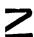
\includegraphics[keepaspectratio]{images/part001_a9d92cc3.jpg}}

显然 n 包含该表示的核。当 M 半单时（命题 4 (c)），n 等于该核，但一般并非如此。应注意，g 中满足 \(x_{M}\) 幂零的元素 x 不一定属于 n。

还要指出，引理 3 的一个特殊情形立即给出以下结果：

命题 5。设 \(\mathbf{V}\) 是 \(n\) 上维数为 \(\mathbf{K}\) 的向量空间，\(g\) 是 \(\mathfrak{gl}(\mathbf{V})\) 的李子代数，且其元素都是 \(\mathbf{V}\) 的幂零自同态。则存在递降的向量子空间序列 \(\mathrm{V}_0, \mathrm{V}_1, \ldots, \mathrm{V}_n\)（其均为 \(\mathbf{V}\) 的子空间），维数为 \(n, n - 1, \ldots, 0\)，使得 \(x(\mathrm{V}_i) \subset \mathrm{V}_{i+1}\) 对所有 \(x \in g\) 及 \(i = 0, 1, \ldots, n - 1\) 成立。

\subsection{李代数的最大幂零理想}

设 \(\mathfrak{g}\) 是李代数，\(\mathfrak{a}\) 是 \(\mathfrak{g}\) 的理想。\(\mathfrak{a}\) 幂零的充要条件是：对所有 \(x \in \mathfrak{a}\)，\(\mathrm{ad}_{\mathfrak{g}}x\) 都是幂零的；充分性显然，而必要性是因为若 \(\mathfrak{a}\) 幂零且 \(x \in \mathfrak{a}\)，则 \(\mathrm{ad}_{\mathfrak{a}}x\) 是幂零的，且 \(\mathrm{ad}_{\mathfrak{a}}x\) 将 \(\mathfrak{g}\) 映入 \(\mathfrak{a}\)，所以 \(\mathrm{ad}_{\mathfrak{g}}x\) 是幂零的。将命题 4 应用于 \(\mathfrak{g}\) 的伴随表示，得到以下结果：

命题 6. 设 \(\mathfrak{g}\) 是李代数，E 是由 1 和 \(\mathcal{L}(\mathfrak{g})\) 生成的 \(\operatorname{ad}_{\mathfrak{g}}x(x\in \mathfrak{g})\) 的结合子代数。令 R 为 E 的 Jacobson 根。

\begin{enumerate}
\def\labelenumi{(\alph{enumi})}
\item
  满足 \(\mathfrak{n}\) 的 \(y\in \mathfrak{g}\) 的集合 \(\operatorname {ad}_{\mathfrak{g}}y\in \mathbb{R}\) 是 \(\mathfrak{g}\) 的最大幂零理想。
\item
  它关于 Killing 形式与 g 正交。
\end{enumerate}

应注意，g/n 可能有非零幂零理想。

\subsection{基域扩张}

设 \(\mathfrak{g}\) 是 K 上的李代数，\(\mathrm{K}_1\) 是 K 的扩域，\(\mathfrak{g}' = \mathfrak{g}_{(\mathrm{K}_1)}\)。由于 \(\mathcal{C}^k\mathfrak{g}' = (\mathcal{C}^k\mathfrak{g})_{(\mathrm{K}_1)}\)，\(\mathfrak{g}\) 幂零当且仅当 \(\mathfrak{g}'\) 幂零。

设 M 是在 K 上有限维的 g-模，n 是 M 的最大幂零理想，且 \(M' = M_{(K_1)}\)。设 \((\mathrm{M}_i)_{0 \leq i \leq n}\) 是 g-模 M 的 Jordan-Hölder 序列。则对所有 i 及所有 \(x_{\mathrm{M}}(\mathrm{M}_i) \subset \mathrm{M}_{i+1}\)，有 \(x \in n\)，因此

\[
x _ {\mathbf {M} ^ {\prime}} ^ {\prime} \left(\left(\mathrm{M} _ {i}\right) _ {\left(\mathrm{K} _ {1}\right)}\right) \subset \left(\mathrm{M} _ {i + 1}\right) _ {\left(\mathrm{K} _ {1}\right)}
\]

对所有 \(i\) 及所有 \(x' \in \mathfrak{n}_{(\mathbf{K}_1)}\) 成立；因此当 \(x_{\mathbf{M}}'\) 时 \(x' \in \mathfrak{n}_{(\mathbf{K}_1)}\) 是幂零的，从而 \(\mathfrak{n}_{(\mathbf{K}_1)}\) 包含于 \(\mathfrak{n}'\) 的最大幂零理想 \(\mathbf{M}'\)。现在证明：若 \(\mathbf{K}_1\) 在 \(\mathbf{K}\) 上可分，则 \(\mathfrak{n}' = \mathfrak{n}_{(\mathbf{K}_1)}\)。令 \(\mathbf{E}\) 为由 1 和 \(\mathbf{x}_{\mathbf{M}}\)（\(x \in \mathfrak{g}\)）生成的结合 K-代数，E' 为由 1 和 \(\mathbf{x}_{\mathbf{M}}\)（\(x' \in \mathfrak{g}'\)）生成的结合 K-代数，\(\mathbf{R}\) 和 \(\mathbf{R}'\) 分别为 \(\mathbf{E}\) 和 \(\mathbf{E}'\) 的 Jacobson 根。代数 E' 典范地等同于 \(\mathrm{E}_{(\mathbf{K}_1)}\)。于是 \(\mathrm{R}' = \mathrm{R}_{(\mathbf{K}_1)}\)（《代数》，第 VIII 章，§ 7，第 2 号命题 3 的推论 2 (c)）。现在令 \(y' \in \mathfrak{n}'\)，写成 \(y^{\prime} = \sum_{i = 1}^{n}\lambda_{i}y_{i}\)，其中 \(y_{i}\) 属于 \(\mathfrak{g}\)，且 \(\lambda_{i}\in \mathrm{K}_{1}\) 在 K 上线性无关。于是 \(y_{\mathbf{M}'}' = \sum_{i=1}^{n} \lambda_i(y_i)_{\mathbf{M}'}\)，并且 \(y_{\mathbf{M}'}' \in \mathbb{R}' = \mathbb{R}_{(\mathbf{K}_1)}\)。所以 \((y_i)_{\mathbf{M}} \in \mathbb{R}\)，从而对所有 \(y_i \in \mathfrak{n}\) 有 \(i\)。因此 \(y' \in \mathfrak{n}_{(\mathbf{K}_1)}\)，即 \(\mathfrak{n}' \subset \mathfrak{n}_{(\mathbf{K}_1)}\)。

特别地，若 \(\mathbf{K}_1\) 在 \(\mathbf{K}\) 上可分，则 \(\mathfrak{g}_{(\mathbf{K}_1)}\) 的最大幂零理想由 \(\mathfrak{g}\) 的最大幂零理想通过将基域从 \(\mathbf{K}\) 扩张到 \(\mathbf{K}_1\) 而得到。

\section{可解李代数}

回顾一下，以下 K 均表示特征为 0 的域，并且所有李代数均假定在 K 上有限维。†

\subsection{可解李代数的定义}

定义 1。若李代数 g 的第 \(\mathcal{D}^{k}\mathfrak{g}\) 个导出代数 \(k\) 在 k 充分大时为零，则称 g 是可解的。

幂零李代数是可解的。

命题 1. 可解李代数的子代数和商代数都是可解的。可解代数由可解代数扩张得到的每个扩张都是可解的。有限个可解代数的直积也是可解的。

设 g 是李代数，\(g'\) 是子代数，h 是 g 的理想，t = g/h，\(\phi\) 是从 g 到 t 的典范映射。若 g 可解，则对某个整数 k 有 \(D^{k}g = \{0\}\)，从而 \(D^{k}g' \subset D^{k}g = \{0\}\)，\(D^{k}t = \phi(\mathcal{D}^{k}g) = \{0\}\)，所以 \(g'\) 和 t 都可解。若 h 和 t 可解，则存在整数 s、t，使得

\[
\mathcal {D} ^ {s} \mathfrak {h} = \mathcal {D} ^ {t} \mathfrak {k} = \{0 \};
\]

则 \(\mathcal{D}^t\mathfrak{g}\subset \mathfrak{h}\)，从而 \(\mathcal{D}^{s + t}\mathfrak{g} = \mathcal{D}^{s}(\mathcal{D}^{t}\mathfrak{g})\subset \mathcal{D}^{s}\mathfrak{h} = \{0\}\)，且 \(\mathfrak{g}\) 可解。最后一个断言由第二个断言对因子个数作归纳得到。

命题 2. 设 g 是李代数。以下条件等价：

\begin{enumerate}
\def\labelenumi{(\alph{enumi})}
\item
  g 是可解的；
\item
  存在 \(\mathfrak{g} = \mathfrak{g}_0 \supset \mathfrak{g}_1 \supset \dots \supset \mathfrak{g}_n = \{0\}\) 的理想递降序列 \(\mathfrak{g}\)，使得代数 \(\mathfrak{g}_i / \mathfrak{g}_{i+1}\) 是交换的（\(i = 0, 1, \ldots, n-1\)）；
\item
  存在 \(\mathfrak{g} = \mathfrak{g}_0' \supset \mathfrak{g}_1' \supset \dots \supset \mathfrak{g}_p' = \{0\}\) 的子代数递降序列 \(\mathfrak{g}\)，使得 \(\mathfrak{g}_{i+1}'\) 是 \(\mathfrak{g}_i'\) 的理想且 \(\mathfrak{g}_i'/\mathfrak{g}_{i+1}'\) 是交换的（\(i = 0, 1, \ldots, p - 1\)）；
\item
  存在 \(\mathfrak{g} = \mathfrak{g}_0'' \supset \mathfrak{g}_1'' \supset \dots \supset \mathfrak{g}_q'' = \{0\}\) 的子代数递降序列 \(\mathfrak{g}\)，使得 \(\mathfrak{g}_{i+1}''\) 是 \(\mathfrak{g}_i''\) 的余维 1 理想（\(i = 0, 1, \ldots, q - 1\)）。
\item
  \(\Rightarrow\) (b)：只需考虑 g 的导出理想序列。
\item
  \(\Rightarrow\) (c)：显然。
\item
  \(\Rightarrow\) (d)：假设条件 (c) 成立；\(\mathfrak{g}_i'\) 中每个包含 \(\mathfrak{g}_{i+1}'\) 的向量子空间都是 \(\mathfrak{g}_i'\) 的理想，故 (d) 立即成立。
\item
  \(\Rightarrow\) (a)：这立即由可解代数由可解代数扩张所得的扩张仍可解这一事实得到。
\end{enumerate}

\subsection*{可解李代数的例子}

I. 设 g 是 K 上的二维向量空间，\((e_{1}, e_{2})\) 是 g 的一组基。g 上存在唯一的交错双线性乘法 \((x, y) \mapsto [x, y]\)，使得 \([e_{1}, e_{2}] = e_{2}\)。容易验证，这样 g 就成为可解李代数。现在设 h 是 K 上二维的非交换李代数。我们证明 h 同构于 g。设 \((f_{1}, f_{2})\) 是 h 的一组基。元素 \([f_{1}, f_{2}]\) 非零（否则 h 将交换），因而它生成 h 的一维子空间 t。于是 \([h, h] = t\)。设 \((e_{1}^{\prime}, e_{2}^{\prime})\) 是 h 的一组基，且 \(e_{2}^{\prime} \in t\)。则 \([e_{1}^{\prime}, e_{2}^{\prime}] = \lambda e_{2}^{\prime}\)，其中 \(\lambda \neq 0\)。将 \(e_{1}^{\prime}\) 替换为 \(\lambda^{-1}e_{1}\)，可设 \(\lambda = 1\)，从而得到所述断言。

\begin{enumerate}
\def\labelenumi{\Roman{enumi}.}
\setcounter{enumi}{1}
\tightlist
\item
  §1 的公式 (5) 证明了 \(\mathcal{D}t(n, \mathbf{K}) = \mathfrak{n}(n, \mathbf{K})\)。由于 \(\mathfrak{n}(n, \mathbf{K})\) 是幂零的，因而可解，\(t(n, \mathbf{K})\) 是可解的。因此 \(\operatorname{st}(n, \mathbf{K})\) 是可解的。特别地，\(\operatorname{st}(2, \mathbf{K})\) 同构于例 I 中的代数。
\end{enumerate}

\subsection{李代数的根基}

设 \(a, b\) 是李代数 \(g\) 的两个可解理想。代数 \((a + b)/b\) 同构于 \(a/(a \cap b)\)，因而是可解的；而 \(a + b\) 是由 \((a + b)/b\) 扩张 \(b\) 得到的扩张，所以也是可解的（命题 1）。由此可知，\(g\) 的一个极大可解理想包含 \(g\) 的每个可解理想，因而 \(g\) 有最大可解理想。这使我们可以作如下定义：

定义 2. 李代数的根基是它的最大可解理想。

命题 3. 李代数 \(\mathfrak{r}\) 的根基 \(\mathfrak{g}\) 是 \(\mathfrak{g}\) 的最小理想，使得 \(\mathfrak{g} / \mathfrak{r}\) 的根基为 \(\{0\}\)。

设 \(\mathfrak{a}\) 是 \(\mathfrak{g}\) 的一个理想，\(\phi\) 是将 \(\mathfrak{g}\) 映到 \(\mathfrak{g}/\mathfrak{a}\) 上的典范映射。若 \(\mathfrak{g}/\mathfrak{a}\) 的根基为零，则 \(\phi(\mathfrak{r})\) 是 \(\mathfrak{g}/\mathfrak{a}\) 的可解理想，因而为零；所以 \(\mathfrak{r} \subset \mathfrak{a}\)。另一方面，\(\overline{\phi}^{-1}(\mathfrak{r}')\) 的根基 \(\mathfrak{r}'\) 的逆像 \(\mathfrak{g}/\mathfrak{r}\) 是 \(\mathfrak{g}\) 的理想，根据命题 1 它是可解的，因而等于 \(\mathfrak{r}\)；所以 \(\mathfrak{r}' = \{0\}\)。

命题 4。设 \(\mathfrak{g}_1, \ldots, \mathfrak{g}_n\) 是李代数。各 \(\mathfrak{r}\) 的乘积的根基 \(\mathfrak{g}_i\) 等于各 \(\mathfrak{r}_i\) 的根基 \(\mathfrak{g}_i\) 的乘积。

各 \(\mathfrak{r}'\) 的乘积 \(\mathfrak{r}_i\) 是一个可解理想（命题 1），因而 \(\mathfrak{r}' \subset \mathfrak{r}\)。\(\mathfrak{r}\) 在 \(\mathfrak{g}_i\) 中的典范像是 \(\mathfrak{g}_i\) 的可解理想，因而包含于 \(\mathfrak{r}_i\)；所以 \(\mathfrak{r} \subset \mathfrak{r}'\)。

\subsection{李代数的幂零根基}

定义 3。设 g 是李代数。g 的幂零根基是 g 的有限维简单表示的核的交。

注记。（1）设 \(\mathfrak{s}\) 是 \(\mathfrak{g}\) 的幂零根基。由于 \(\mathfrak{g}\) 的向量子空间的每个递降序列都稳定，所以存在有限个 \(\mathfrak{g}\) 的有限维简单表示，其核的交为 \(\mathfrak{s}\)。

这些表示的直和是半单的，且其核为 s。因此，g 的有限维半单表示的核所成的集合有最小元，即 s。

\begin{enumerate}
\def\labelenumi{(\arabic{enumi})}
\setcounter{enumi}{1}
\item
  根据 §4 第 3 号的命题 4 (c)，s 也是 g 的有限维表示的最大幂零理想的交。特别地，s 包含于 g 的最大幂零理想中，因而是 g 的幂零理想。
\item
  每个线性形式 \(\lambda\) 在 \(\mathfrak{g}\) 上且在 \(\mathcal{D}\mathfrak{g}\) 上为零；它都是以 \(\mathbf{K}\) 为表示空间的 \(\mathfrak{g}\) 的简单表示，从而 \(\lambda (\mathfrak{s}) = \{0\}\)。因此 \(\mathfrak{s} \subset \mathcal{D}\mathfrak{g}\)。另一方面，由注记 2，\(\mathfrak{s}\) 包含于 \(\mathfrak{r}\) 的根基 \(\mathfrak{g}\) 中。我们将证明 \(\mathfrak{s} = \mathfrak{r} \cap \mathcal{D}\mathfrak{g}\)。
\end{enumerate}

引理 1. 设 \(\mathbf{V}\) 是 \(\mathbf{K}\) 上的有限维向量空间，\(\mathfrak{g}\) 是 \(\mathfrak{gl}(\mathbf{V})\) 的子代数，使得 \(\mathbf{V}\) 是简单的 \(\mathfrak{g}\)-模，\(\mathfrak{a}\) 是 \(\mathfrak{g}\) 的交换理想。则 \(\mathfrak{a} \cap \mathcal{D}\mathfrak{g} = \{0\}\)。令 \(\mathbf{S}\) 为由 1 和 \(\mathcal{L}(\mathbf{V})\) 生成的 \(\mathfrak{a}\) 的子代数。

若 \(\mathfrak{b}\) 是 \(\mathfrak{g}\) 中包含于 \(\mathfrak{a}\) 的理想，且对所有 \(\operatorname{Tr}bs = 0\) 及所有 \(b\in \mathfrak{b}\) 有 \(s\in S\)，则特别地，根据 \(S\) 的定义，对每个整数 \(\operatorname{Tr}(b^n) = 0\) 有 \(n > 0\)，从而 \(b\) 是幂零的（《代数》，第 VII 章，§ 5，第 5 号，命题 13 的推论 4）；由于 \(\mathfrak{b}\) 的元素全都是幂零的，\(\mathfrak{b} = \{0\}\)（§ 4，第 3 号，引理 2）。我们首先将此应用于 \([\mathfrak{g},\mathfrak{a}]\) 的理想 \(\mathfrak{g}\)。若 \(x\in \mathfrak{g}\)、\(a\in \mathfrak{a}\)、\(s\in S\)，则 \(\operatorname{Tr}[x,a]s = \operatorname{Tr}(xas - axs) = \operatorname{Tr}x(as - sa) = 0\)，因为 \(as = sa\)；所以 \([\mathfrak{g},\mathfrak{a}] = \{0\}\)。因此 \(\mathfrak{g}\) 的元素与 \(\mathfrak{a}\) 的元素可交换，因而也与 \(S\) 的元素可交换。若 \(x,y\) 属于 \(\mathfrak{g}\) 且 \(s\in S\)，则

\[
\operatorname{Tr} [ x, y ] s = \operatorname{Tr} (x y s - y x s) = \operatorname{Tr} x (y s - s y) = 0
\]

由于 \(ys = sy\)，取 \(b\) 为理想 \(\mathcal{D}\mathfrak{g} \cap a\)，便得到 \(\mathcal{D}\mathfrak{g} \cap a = \{0\}\)。

定理 1. 设 \(\mathfrak{g}\) 是李代数，\(\mathfrak{r}\) 是其根基，\(\mathfrak{s}\) 是其幂零根基。则 \(\mathfrak{s} = \mathcal{D}\mathfrak{g} \cap \mathfrak{r}\)。

我们已经知道 \(\mathfrak{s} \subset \mathcal{D}\mathfrak{g} \cap \mathfrak{r}\)。因此只需证明：若 \(\rho\) 是 \(\mathfrak{g}\) 的有限维简单表示，则 \(\rho(\mathcal{D}\mathfrak{g} \cap \mathfrak{r}) = \{0\}\)。令 \(k\) 是最小的、\(\geqslant 0\) 且使 \(\rho(\mathcal{D}^{k}\mathfrak{r}) = \{0\}\) 的整数；记 \(\mathfrak{g}' = \rho(\mathfrak{g})\)、\(\mathfrak{a}' = \rho(\mathrm{D}^k\mathfrak{r})\)；由于 \(\mathcal{D}^k\mathfrak{r}\) 是 \(\mathfrak{g}\) 的理想，\(\mathfrak{a}'\) 是 \(\mathfrak{g}'\) 的理想；由于 \(\rho(\mathcal{D}^{k}\mathfrak{r}) = \{0\}\)，这个理想是交换的。若 \(\mathrm{V}\) 是 \(\rho\) 的表示空间，则 \(\mathfrak{g}' \subset \mathfrak{gl}(\mathrm{V})\)，且 \(\mathrm{V}\) 是简单的 \(\mathfrak{g}'\)-模。于是 \(\rho(\mathcal{D}\mathfrak{g} \cap \mathcal{D}^k\mathfrak{r}) \subset \mathcal{D}\mathfrak{g}' \cap \mathfrak{a}' = \{0\}\)。若 \(k > 0\)，则 \(\mathcal{D}^k\mathfrak{r} \subset \mathcal{D}\mathfrak{g}\) 且 \(\rho(\mathcal{D}^k\mathfrak{r}) = \{0\}\)，这与 k 的定义矛盾。因此 \(k\) 为 \(k = 0\)，即

\[
\rho (\mathcal{D}\mathfrak{g} \cap \mathfrak{r}) = \{0 \}.
\]

推论 1. 设 g 是可解李代数。g 的幂零根基是 \(\mathcal{D}\mathfrak{g}\)。若 \(\rho\) 是 g 的有限维简单表示，则 \(\rho(\mathfrak{g})\) 是交换的，并且由 1 和 \(\rho(\mathfrak{g})\) 生成的结合代数 L 是 K 的有限次扩域。

这里 \(\mathfrak{r} = \mathfrak{g}\)，从而 \(\mathfrak{s} = \mathcal{D}\mathfrak{g}\)。所以 \(\rho(\mathcal{D}\mathfrak{g}) = \{0\}\)，这说明 \(\mathfrak{g}' = \rho(\mathfrak{g})\) 是交换的。根据 Schur 引理，\(\neq 0\) 的每个 \(\mathbf{L}\) 元素都是可逆的；所以 \(\mathbf{L}\) 是域。

推论 2（李定理）. 设 \(\mathfrak{g}\) 是可解李代数；假设 \(\mathbf{K}\) 代数闭。令 \(\mathbf{M}\) 是在 \(\mathfrak{g}\) 上有限维的 \(\mathbf{K}\)-模，\((\mathrm{M}_1)_{0 \leqslant i \leqslant r}\) 是 \(\mathbf{M}\) 的 Jordan-Hölder 序列。则对 \(\mathrm{M}_{i - 1} / \mathrm{M}_i\)，\(\mathbf{K}\) 在 \(1 \leqslant i \leqslant r\) 上的维数为 1，并且对所有 \(x \in \mathfrak{g}\)，有 \(x_{\mathrm{M}_{i - 1} / \mathrm{M}_i} = \lambda_i(x)\) . 1，其中 \(\lambda_i\) 是 \(\mathfrak{g}\) 上在 \(\mathcal{D}\mathfrak{g}\) 上为零的线性形式。特别地，每个在 \(\mathfrak{g}\) 上有限维的简单 \(\mathbf{K}\)-模实际上都是一维的。

令 \(\rho_{i}\) 是 \(g\) 在 \(\mathbf{M}_{i-1}/\mathbf{M}_{i}\) 上的表示。由 1 和 \(\mathbf{L}_{i}\) 生成的结合代数 \(\rho_{i}(g)\) 是域，是 K 的有限扩域，因而等于 K；而 \(\mathbf{M}_{i-1}/\mathbf{M}_{i}\) 是简单的 \(\mathbf{L}_{i}\)-模，所以 \(\dim \mathbf{M}_{i-1}/\mathbf{M}_{i} = 1\)。推论的其余部分显然。

注记。（1）若 \((\mathrm{M}_i)_{0\leqslant i\leqslant r}\) 被 M 的另一个 Jordan-Hölder 序列替代，则序列 \((\lambda_1,\dots ,\lambda_r)\) 被形如 \((\lambda_{\pi (1)},\dots ,\lambda_{\pi (r)})\) 的序列替代，其中 \(\pi\) 是 \(\{1,\dots ,r\}\) 的一个置换；这是 Jordan-Hölder 定理的结果。

\begin{enumerate}
\def\labelenumi{(\arabic{enumi})}
\setcounter{enumi}{1}
\tightlist
\item
  设 \((e_1, \ldots, e_r)\) 是 M 的一组基，满足 \(e_i \in \mathbf{M}_{i-1}, e_i \notin \mathbf{M}_i\)、\(1 \leqslant i \leqslant r\)（\(x \in \mathfrak{g}\)）。若 \(x\)，则相应于 x 的 M 的自同态相对于此基由一个三角矩阵表示，其对角系数为
\end{enumerate}

\[
\lambda_ {1} (x), \dots , \lambda_ {\tau} (x).
\]

推论 3. 假设 K 代数闭。若 g 是 r 维可解李代数，则 g 的每个理想都是维数为 r、r - 1、\ldots、0 的理想递降序列中的一项。

每个理想都是 g（看作伴随表示的表示空间）的一个 Jordan-Hölder 序列的一部分（《代数》，第 I 章，§ 6，第 14 号，定理 8 的推论）；因此只需应用推论 2。

推论 4. 假设 \(\mathbf{K} = \mathbf{R}\)。设 \(\mathfrak{g}\) 是可解李代数。每个 \(\mathfrak{g}\) 的简单表示的维数都 \(\leqslant 2\)。\(\mathfrak{g}\) 的每个理想都是理想递降序列 \((\mathfrak{g}_i)_{0\leqslant i\leqslant m}\) 中的一项，其中 \(\mathfrak{g}_0 = \mathfrak{g},\mathfrak{g}_m = \{0\}\)，且 \(\dim \mathfrak{g}_{i - 1} / \mathfrak{g}_i\leqslant 2\)（\(1\leqslant i\leqslant m\)）。

证明方式与推论 2、3 的证明类似，只需使用每个 \(\mathbf{R}\) 的代数扩域的次数都 \(\leqslant 2\) 这一事实。

推论 5. 李代数 g 可解的充要条件是 \(\mathcal{D}\mathfrak{g}\) 幂零。

必要性由推论 1 得到。充分性成立是因为 \(\mathfrak{g} / \mathcal{D}\mathfrak{g}\) 是交换的。

推论 6. 设 \(\rho\) 是李代数 \(\mathfrak{g}\) 的有限维表示。设 \(\mathfrak{r}\) 是 \(\mathfrak{g}\) 的根基。每个满足 \(x \in \mathfrak{r}\) 幂零的 \(\rho(x)\) 都属于 \(\mathfrak{n}\) 的最大幂零理想 \(\rho\)。

设 \(V\) 是 \(\rho\) 的表示空间；令 \(\langle V_i \rangle_{0 \leqslant i \leqslant r}\) 是 \(r\)-模结构在 \(V\) 上的 Jordan-Hölder 序列，并令 \(\rho_i\) 是 \(r\) 在 \(V_i / V_{i-1}\) 上的表示（\(1 \leqslant i \leqslant r\)）。若 \(\rho(x)\) 是幂零的，则 \(\rho_i(x)\) 也是幂零的；因为对所有 \(i\)，由 \(\rho_i(x)\) 生成的代数是域，所以 \(\rho_i(x) = 0\)。反之，若 \(\rho_i(x) = 0\)，则对所有 \(i, \rho(x) = 0\) 都成立。这说明集合 \(a\) 中满足 \(x \in r\) 且 \(\rho(x)\) 幂零的元素是 \(r\) 的理想。另一方面，\([g, a] \subset \mathcal{D}g \cap r \subset n \cap r \subset a\)，所以 \(a\) 是 \(g\) 的理想。这证明了 \(a \subset n\)。

推论 7. 设 g 是李代数，r 是其根基。以下四个集合相同：(a) g 的最大幂零理想；(b) r 的最大幂零理想；(c) 满足 \(x \in \mathfrak{r}\) 幂零的 \(\operatorname{ad}_{\mathfrak{g}} x\) 的集合；(d) 满足 \(x \in \mathfrak{r}\) 幂零的 \(\operatorname{ad}_{\mathfrak{r}} x\) 的集合。

将这些集合记为 \(\mathfrak{a}, \mathfrak{b}, \mathfrak{c}, \mathfrak{d}\)。包含关系 \(\mathfrak{a} \subset \mathfrak{b} \subset \mathfrak{d} \subset \mathfrak{c}\) 显然。由推论 6 应用于 \(\mathfrak{c} \subset \mathfrak{a}\) 的伴随表示，得 \(\mathfrak{g}\)。

\subsection{可解性的判据}

引理 2。设 \(x\) 是有限维向量空间 \(V\) 的自同态，\(s\)（分别 \(n\)）是其半单（分别幂零）分量（参见《代数》，第 VIII 章，§ 9，第 4 号，定义 4）。令 \(ad_x\)、\(ad_s\)、\(ad_n\) 分别为 \(x\)、\(s\)、\(n\) 在 \(gl(V)\) 的伴随表示下的像。则 \(ad_s\)（分别 \(ad_n\)）是 \(ad_x\) 的半单（分别幂零）分量，并且等于 \(ad_x\) 中系数在 \(K\) 内且无常数项的一个多项式。

我们知道 \(\operatorname{ad} x = \operatorname{ad} s + \operatorname{ad} n\)，\([\operatorname{ad} s, \operatorname{ad} n] = 0\)，且 \(\operatorname{ad} n\) 是幂零的（§ 4，引理 1）。我们证明 \(\operatorname{ad} s\) 是半单的。只需在 \(\mathbf{K}\) 代数闭时证明即可（参见《代数》，第 VIII 章，§ 9，第 2 号，命题 3）。令 \((e_i)_{1 \leq i \leq n}\) 是 \(V\) 的一组基，满足 \(s(e_i) = \lambda_i e_i\)（\(\lambda_i \in K\)）。令 \((E_{ij})\) 是 \(\mathbf{M}_n(K) = \mathfrak{gl}(V)\) 的典范基。由 § 1 的公式 (5)，

\[
(\mathrm{ad} s). E _ {i j} = (\lambda_ {i} - \lambda_ {j}) E _ {i j}
\]

从而 ad s 是半单的。引理的最后一个断言由《代数》第 VIII 章 § 9 第 4 号命题 8 得到。

引理 3。设 \(\mathbf{M}\) 是有限维向量空间，\(\mathbf{A}\)、\(\mathbf{B}\) 是 \(\mathfrak{gl}(\mathbf{M})\) 的两个向量子空间，满足 \(\mathbf{B} \subset \mathbf{A}\)，\(\mathbf{T}\) 是满足 \(t \in \mathfrak{gl}(\mathbf{M})\) 且 \([t, \mathbf{A}] \subset \mathbf{B}\) 的 t 的集合。若 \(z \in \mathbf{T}\) 且对所有 \(\operatorname{Tr}(zu) = 0\) 有 \(u \in \mathbf{T}\)，则 \(z\) 是幂零的。

只需在 \(\mathbf{K}\) 代数闭时证明这一点，以下均作此假设。令 \(s\) 和 \(n\) 是 \(z\) 的半单分量和幂零分量，令 \((e_i)\) 是 \(\mathbf{M}\) 的一组基，满足 \(s(e_i) = \lambda_i e_i\)（\(\lambda_i \in \mathbf{K}\)）。令 \(\mathbf{V} \subset \mathbf{K}\) 是由 \(\mathbf{Q}\) 生成的、包含 \(\lambda_i\) 的向量空间。我们需要证明 \(\mathbf{V} = \{0\}\)。令 \(f\) 是 \(\mathbf{Q}\) 上的 \(\mathbf{V}\)-线性形式，令 \(t\) 是 \(\mathbf{M}\) 的自同态，满足 \(te_{i}=f(\lambda_{i})e_{i}\)。若 \((E_{ij})\) 是由 \(E_{ij}e_{k}=\delta_{jk}e_{i}\) 定义的 gl(M) 的典范基，则

\[
\begin{array}{l} (\mathrm{ad} s) E _ {i j} = (\lambda_ {i} - \lambda_ {j}) E _ {i j} \\ (\mathrm{ad} t) E _ {i j} = (f (\lambda_ {i}) - f (\lambda_ {j})) E _ {i j}. \end{array}
\]

存在一个无常数项且系数在 \(\mathbf{P}\) 中的多项式 \(\mathbf{K}\)，使得 \(\mathrm{P}(\lambda_i - \lambda_j) = f(\lambda_i) - f(\lambda_j)\) 对所有 \(i\) 和 \(j\) 成立（因为若 \(\lambda_i - \lambda_j = \lambda_h - \lambda_k\)，则 \(f(\lambda_i) - f(\lambda_j) = f(\lambda_h) - f(\lambda_k)\)），并且当 \(\lambda_i - \lambda_j = 0\) 时，\(f(\lambda_i) - f(\lambda_j) = 0\)。于是 \(t = \mathrm{P}(\mathrm{ad}s)\)。另一方面，ad \(s\) 是 ad \(z\) 中一个无常数项的多项式。现在 ad \(z\)(A) \(\subset \mathrm{B}\)，所以 ad \(t\)(A) \(\subset \mathrm{B}\)。根据假设 \(0 = \operatorname{Tr}(zt) = \sum_{\lambda_i} f(\lambda_i)\)，从而 \(0 = f(\operatorname{Tr}(zt)) = \sum f(\lambda_i)^2\)。由于 \(f(\lambda_i)\) 是有理数，\(f = 0\)，证明完成。

定理 2（Cartan 判据）. 设 \(\mathfrak{g}\) 是李代数，\(\mathbf{M}\) 是有限维向量空间，\(\rho\) 是 \(\mathfrak{g}\) 在 \(\mathbf{M}\) 上的表示，\(\beta\) 是与 \(\mathfrak{g}\) 关联的 \(\rho\) 上的双线性形式。则 \(\rho(\mathfrak{g})\) 可解，当且仅当 \(\mathcal{D}\mathfrak{g}\) 关于 \(\mathfrak{g}\) 与 \(\beta\) 正交。

显然可将问题化为 \(\mathfrak{g}\) 是 \(\mathfrak{gl}(\mathbf{M})\) 的李子代数且 \(\rho\) 是恒等映射的情形。若 \(\mathfrak{g}\) 可解，则由定理 1，\(\mathcal{D}\mathfrak{g}\) 包含于恒等表示的 \(\mathfrak{g}\) 的最大幂零理想中，因而是关于 \(\mathfrak{g}\) 与 \(\beta\) 正交（\(\S 4\)，命题 4 (d)）。假设 \(\mathcal{D}\mathfrak{g}\) 关于 \(\mathfrak{g}\) 与 \(\beta\) 正交。我们证明 \(\mathfrak{g}\) 可解。令 \(\mathrm{T}\) 为满足 \(t\in \mathfrak{gl}(\mathbf{M})\) 且 \([t,\mathfrak{g}]\subset \mathcal{D}\mathfrak{g}\) 的 t 的集合。若 \(t\in \mathrm{T}\) 且 \(x,y\) 属于 \(\mathfrak{g}\)，则 \([t,x]\in \mathcal{D}\mathfrak{g}\)，所以

\[
\operatorname{Tr} (t [ x, y ]) = \beta ([ t, x ], y) = 0
\]

由线性性，对所有 \(\mathrm{Tr}(tu) = 0\) 有 \(u\in \mathcal{D}\mathfrak{g}\)。显然 \(\mathcal{D}\mathfrak{g}\subset T\)。因此（引理 3），\(\mathcal{D}\mathfrak{g}\) 的每个元素都是幂零的。于是 \(\mathcal{D}\mathfrak{g}\) 是幂零的（§ 4，定理 1 的推论 3），从而 \(\mathfrak{g}\) 可解（第 3 号，定理 1 的推论 5）。

\subsection{根基的进一步性质}

命题 5. 设 g 是李代数，r 是其根基。

\begin{enumerate}
\def\labelenumi{(\alph{enumi})}
\item
  如果 \(\rho\) 是 \(\mathfrak{g}\) 的有限维表示，\(\beta\) 是相应的双线性形式，则 \(\mathfrak{r}\) 和 \(\mathcal{D}\mathfrak{g}\) 关于 \(\beta\) 正交。
\item
  r 关于 Killing 形式是 \(\mathcal{D}\mathfrak{g}\) 的正交子空间。
\end{enumerate}

设 \(x, y\) 属于 \(\mathfrak{g}, z \in \mathfrak{r}\)。则 \([y, z] \in \mathcal{D}\mathfrak{g} \cap \mathfrak{r}\)，所以

\[
\beta ([ x, y ], z) = \beta (x, [ y, z ]) = 0
\]

（定理 1）。所以 (a)。

令 \(\mathfrak{r}'\) 是 \(\mathcal{D}\mathfrak{g}\) 关于 Killing 形式的正交子空间。它是 \(\mathfrak{g}\) 的理想（\(\S 3\)，第 6 号，命题 7 (a)），由上面所述包含 \(\mathfrak{r}\)。另一方面，\(\mathfrak{r}'\) 在 \(\mathfrak{g}\) 的伴随表示下的像 s 是可解的（定理 2），所以 \(\mathfrak{r}'\) 是可解的，因为它是 s 的中心扩张。因此 \(\mathfrak{r}' \subset \mathfrak{r}\)。

推论 1. 设 \(\mathfrak{g}\) 是李代数。则 \(\mathfrak{g}\) 可解，当且仅当 \(\mathcal{D}\mathfrak{g}\) 关于 Killing 形式与 \(\mathfrak{g}\) 正交。

这立即由命题 5 (b) 得到。

推论 2. 李代数 \(\mathfrak{r}\) 的根基 \(\mathfrak{g}\) 是特征理想。

\(\mathcal{D}\mathfrak{g}\) 是特征理想，且 Killing 形式是完全不变的（§ 3，第 6 号，命题 10）。因此，\(\mathcal{D}\mathfrak{g}\) 关于 Killing 形式的正交子空间是特征理想（§ 3，第 6 号，命题 7 (b)）。

推论 3。设 g 是李代数，r 是其根基，a 是 g 的理想。则 a 的根基等于 r 与 a 的交。

\(r \cap a\) 是 \(a\) 的可解理想，因而包含于 \(r'\) 的根基 \(a\) 中。反之，\(r'\) 是 \(g\) 的理想（推论 2 以及 §1，第 4 号，命题 2），所以 \(r' \subset r\)。

推论 2 可以精确表述如下：

命题 6. 设 \(\mathfrak{g}\) 是李代数，\(\mathfrak{r}\) 是其根基，\(\mathfrak{n}\) 是其最大幂零理想。每个 \(\mathfrak{g}\) 的导子都将 \(\mathfrak{r}\) 映入 \(\mathfrak{n}\)。

设 D 是 g 的导子。令 \(g' = g + Kx_0\) 是一个李代数，其中 g 是余维 1 的理想，且对所有 \(Dx = [x_0, x]\) 有 \(x \in g\)（§ 1，第 8 号，例 1）。根据命题 5 的推论 3，r 包含于 \(r'\) 的根基 \(g'\) 中。于是 \(D(r) = [x_0, r] \subset [g', g'] \cap r' = s'\)。对所有 \(x \in s' \cup g\)，\(ad_g x\) 都是幂零的（定理 1）。因此，对所有 \(x \in s' \cap g\)，\(ad_g x\) 都是幂零的。所以 \(D(r)\) 包含于 g 的幂零理想 \(s' \cap g\) 中。

推论。李代数的最大幂零理想是特征理想。

注记。总结上述一些结果：若 r、n、s、t 分别表示 g 的根基、g 的最大幂零理想、g 的幂零根基以及 g 关于 Killing 形式的正交子空间，则

\[
\mathfrak {r} \supset \mathfrak {k} \supset \mathfrak {n} \supset \mathfrak {s}.
\]

包含关系 \(\mathfrak{r} \supset \mathfrak{t}\) 由命题 5 (b) 得到。包含关系 \(\mathfrak{t} \supset \mathfrak{n}\) 由 §4，第 4 号，命题 6 (b) 得到。包含关系 \(\mathfrak{n} \supset \mathfrak{s}\) 已在第 3 号的注记 2 中指出。

\subsection{基域扩张}

设 \(\mathfrak{g}\) 是一个 K 上的李代数，\(\mathbf{K}_1\) 是 K 的扩域。显然，\(\mathfrak{g}_{(\mathbf{K}_1)}\) 可解，当且仅当 \(\mathfrak{g}\) 可解，因为 \(\mathcal{D}^n (\mathfrak{g}_{(\mathbf{K}_1)}) = (\mathcal{D}^n\mathfrak{g})_{(\mathbf{K}_1)}\)。

设 \(\mathfrak{r}\) 是 \(\mathfrak{g}\) 的根基。则 \(\mathfrak{r}_{(\mathbf{K}_1)}\) 是 \(\mathfrak{g}_{(\mathbf{K}_1)}\) 的根基。事实上，设 \(\beta\) 是 \(\mathfrak{g}\) 的 Killing 形式。由于 \(\mathfrak{r}\) 是 \(\mathcal{D}\mathfrak{g}\) 关于 \(\beta\) 的正交子空间（命题 5 (b)），\(\mathfrak{r}_{(\mathbf{K}_1)}\) 是 \((\mathcal{D}\mathfrak{g})_{(\mathbf{K}_1)} = \mathcal{D}(\mathfrak{g}_{(\mathbf{K}_1)})\) 关于由 \(\beta\) 从 \(\mathbf{K}\) 扩张到 \(\mathbf{K}_1\) 所得到的形式的正交子空间；该形式就是 \(\mathfrak{g}_{(\mathbf{K}_1)}\) 的 Killing 形式（\(\S 3\)，第 8 号）。我们的断言于是由再次应用命题 5 (b) 得到。

\section{半单李代数}

回顾一下，K 表示特征为 0 的域，且所有李代数均假定在 K 上有限维。

\subsection{半单李代数的定义}

定义 1。设 \(\mathfrak{g}\) 是一个李代数。当且仅当 \(\mathfrak{g}\) 的唯一交换理想是 \(\mathfrak{g}\) 时，称 \(\{0\}\) 为半单的。

注记。（1）零代数 \(\{0\}\) 是半单的。维数为 1 或 2 的代数不是半单的（参见~§ 5，第 1 号，例 1）。存在维数为 3 的半单代数（参见第 7 号）。

\begin{enumerate}
\def\labelenumi{(\arabic{enumi})}
\setcounter{enumi}{1}
\item
  半单代数的中心为零，因而其伴随表示是忠实的。
\item
  若 \(g_{1}, \ldots, g_{n}\) 是半单的，则 \(g = g_{1} \times \cdots \times g_{n}\) 是半单的：因为若 a 是 g 的交换理想，a 在 \(g_{1}, \ldots, g_{n}\) 上的投影都退化为 \(\{0\}\)。
\end{enumerate}

定理 1。设 \(\mathfrak{g}\) 是一个李代数。以下条件等价：

\begin{enumerate}
\def\labelenumi{(\alph{enumi})}
\item
  g 是半单的。
\item
  g 的根基 r 为零。
\item
  \(\beta\) 的 Killing 形式 \(\mathfrak{g}\) 非退化。
\end{enumerate}

此外，半单李代数等于其导出理想。

\begin{enumerate}
\def\labelenumi{(\alph{enumi})}
\item
  \(\Rightarrow\) (b)：因为若 \(\mathfrak{r} \neq \{0\}\)，则 \(\mathfrak{r}\) 的最后一个非零导出代数是 \(\mathfrak{g}\) 的交换理想。
\item
  \(\Rightarrow\) (c)：这由 § 5，第 5 号的命题 5 (b) 得到（这同时证明了定理的最后一个断言）。
\item
  \(\Rightarrow\) (a)：这由 §4，第 4 号的命题 6 (b) 得到。
\end{enumerate}

推论。设 \(\mathfrak{g}\) 是半单李代数，\(\rho\) 是 \(\mathfrak{g}\) 在有限维向量空间 V 上的表示。则 \(\rho(\mathfrak{g}) \subset \mathfrak{sl}(V)\)。

线性形式 \(x \mapsto \operatorname{Tr} \rho(x)\)（\(x \in \mathfrak{g}\)）当 \(x\) 形如 \([y, z]\)（\(y \in \mathfrak{g}, z \in \mathfrak{g}\)）时为零，因而在 \(\mathcal{D}\mathfrak{g} = \mathfrak{g}\) 上也为零。

命题 1。设 \(\mathfrak{g}\) 是半单李代数，\(\rho\) 是 \(\mathfrak{g}\) 的有限维忠实表示。则 \(\mathfrak{g}\) 所关联的 \(\rho\) 上的双线性形式非退化。

该形式关于 g 的正交子空间是一个可解理想（§ 5，第 4 号，定理 2），因而为零。

推论 1。设 g 是一个李代数，\(\beta\) 是其 Killing 形式，\(\mathfrak{a}\) 是 g 的半单子代数。关于 \(\mathfrak{b}\) 与 \(\mathfrak{a}\) 正交的子空间 \(\beta\) 是 g 中 \(\mathfrak{a}\) 的补空间，且 \({[}\mathfrak{a}, \mathfrak{b}{]} \subset \mathfrak{b}\)。若 \(\mathfrak{a}\) 是 g 的理想，则 \(\mathfrak{b}\) 也是理想，此时它是 g 中 \(\mathfrak{a}\) 的中心化子。

设 \(\beta'\) 是 \(\beta\) 在 \(a\) 上的限制：它是 \(x \mapsto \operatorname{ad}_{\mathfrak{g}} x\) 在空间 \(a\) 上由表示 \(\mathfrak{g}\) 所关联的双线性形式。该表示是忠实的，因而 \(\beta'\) 非退化（命题 1）。所以 \(\mathfrak{b}\) 是 \(a\) 在 \(\mathfrak{g}\) 中的补空间。另一方面，若 \(x, y\) 属于 \(a\) 且 \(z \in \mathfrak{b}\)，则

\[
\beta (x, [ y, z ]) = \beta ([ x, y ], z) = 0,
\]

由于 \([x,y] \in \mathfrak{a}\)，所以 \([y,z] \in \mathfrak{b}\)，这证明了 \([\mathfrak{a},\mathfrak{b}] \subset \mathfrak{b}\)。若 \(\mathfrak{a}\) 是 \(\mathfrak{g}\) 的理想，我们知道 \(\mathfrak{b}\) 也是 \(\mathfrak{g}\) 的理想（§ 3，命题 7），且 \(\mathfrak{g}\) 可与 \(\mathfrak{a} \times \mathfrak{b}\) 等同。由于 \(\mathfrak{a}\) 的中心为零，\(\mathfrak{a}\) 中 \(\mathfrak{g}\) 的中心化子是 \(\mathfrak{b}\)。

推论 2。半单李代数的每个半单李代数扩张都是半单的且平凡。

这立即由推论 1 得到。

推论 3。若 g 是半单的，则 g 的每个导子都是内导子。

ad g 同构于 g，因而是半单的，并且是李代数 d（由 g 的导子组成）的理想（§ 1，命题 1）。若 D ∈ d 与 ad g 的元素可交换，则对所有 x ∈ g，有 ad D(x) = {[}D, ad x{]} = 0，从而 D(x) = 0；所以 D = 0。推论 3 现在由推论 1 得到。
